\subsection{\texorpdfstring{Direct Image of a \(\tau\)-Extension}{Direct Image of a \textbackslash tau-Extension}}

Let G be a group, let F and \(F'\) be abelian groups, let \(\tau\) (resp. \(\tau'\) ) be a group homomorphism from G to the automorphism group of F (resp. \(F'\) ), and let \(v: F \to F'\) be a group homomorphism such that

\[
v (\tau (g) \cdot f) = \tau^ {\prime} (g) \cdot v (f)\tag{3}
\]

for every \(g \in G\) and \(f \in F\) . Let \(\mathcal{E} = (\Gamma, \iota, \pi)\) be a \(\tau\) -extension of G by F. Let \(\widetilde{\Gamma}\) be the external semidirect product \(F' \times_{\tau' \circ \pi} \Gamma\) . We denote by \(\widetilde{\iota}: F' \to \widetilde{\Gamma}\) the homomorphism \(f \mapsto (f, e)\) and by \(\widetilde{p}: \widetilde{\Gamma} \to \Gamma\) the first projection. Let \(j: F \to \widetilde{\Gamma}\) be the mapping defined by \(f \mapsto (v(f), \iota(f)^{-1})\) . Since the image of \(\iota\) is contained in the kernel of \(\tau' \circ \pi\) , the mapping j is a group homomorphism; it is injective because \(\iota\) is injective. We have the relations

\[
\begin{array}{r l} (f ^ {\prime}, \gamma) j (f) (f ^ {\prime}, \gamma) ^ {- 1} & = (f ^ {\prime}, \gamma) (v (f), \iota (f) ^ {- 1}) (f ^ {\prime}, \gamma) ^ {- 1} \\ & = (\tau^ {\prime} (\pi (\gamma)) \cdot v (f), \iota (\tau (\pi (\gamma)) \cdot f) ^ {- 1}) \\ & = j (\tau (\pi (\gamma)) \cdot f) \end{array}\tag{4}
\]

for \(f \in F\) , \(\gamma \in \Gamma\) , and \(f' \in F'\) . Consequently, the image of j is a normal subgroup of \(\widetilde{\Gamma}\) . We denote by \(\Gamma'\) the quotient of \(\widetilde{\Gamma}\) by the image of j. We denote by \(\iota'\) the composition of the canonical surjection from \(\widetilde{\Gamma}\) to \(\Gamma'\) and \(\widetilde{\iota}\) . The kernel of the homomorphism \(\pi \circ \widetilde{p}\) is the product \(\mathrm{F}' \times \iota(\mathrm{F})\) , which contains the image of j. We define \(\pi' : \Gamma' \to G\) as the group homomorphism deduced from \(\pi \circ \widetilde{p}\) by passing to the quotient. Since \(\iota\) is injective, the intersection of \(j(\mathrm{F})\) and \(\widetilde{\iota}(\mathrm{F}')\) is reduced to the identity element of \(\widetilde{\Gamma}\) ; it follows that \(\iota'\) is injective. The mapping from \(F' \times F\) to \(F' \times \iota(\mathrm{F}) = \operatorname{Ker}(\pi \circ \widetilde{p})\) given by

\[
(f ^ {\prime}, f) \longmapsto (f ^ {\prime} v (f), \iota (f) ^ {- 1})
\]

is a group isomorphism. The image of \(\iota'\) therefore coincides with the kernel of \(\pi'\) . Since \(\pi\) and \(\widetilde{p}\) are surjective, so is \(\pi'\) . This proves that \(\mathcal{E}' = (\Gamma', \iota, \pi')\) is a \(\tau'\) -extension of \(G\) by \(F'\) ; we call it the direct image of \(\mathcal{E}\) by \(v\) and denote it by \(v_{*}(\mathcal{E})\) . The composition of the canonical surjection from \(\widetilde{\Gamma}\) to \(\Gamma'\) and the group homomorphism from \(\Gamma\) to \(\widetilde{\Gamma}\) given by \(\gamma \mapsto (1, \gamma)\) is a group homomorphism \(\varphi : \Gamma \to \Gamma'\) that we call canonical.

PROPOSITION 2. --- In the notation above, the following diagram commutes:

\begin{enumerate}
\def\labelenumi{(\arabic{enumi})}
\setcounter{enumi}{4}
\tightlist
\item
\end{enumerate}

\pandocbounded{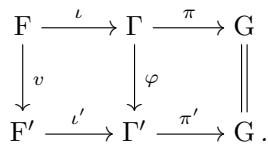
\includegraphics[keepaspectratio]{images/part002_f3abcdb3.jpg}}

Let \(\mathcal{E}_1' = (\Gamma_1', \iota_1', \pi_1')\) be a \(\tau'\) -extension of G by F', and let \(\varphi_1: \Gamma \to \Gamma_1'\) be a group homomorphism such that the following diagram commutes:

\pandocbounded{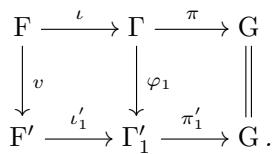
\includegraphics[keepaspectratio]{images/part002_c84edb93.jpg}}

Then there exists a unique morphism \(\psi\) of \(\tau'\) -extensions from \(v_{*}(\mathcal{E})\) to \(\mathcal{E}_1'\) such that we have \(\varphi_1 = \psi \circ \varphi\) .

The commutativity of the first diagram follows by construction. The existence and uniqueness of \(\psi\) follow from Lemma 3 below.

Lemma 3. --- Let \(G_{1}^{\prime}\) be a group, and let \(w: G \to G_{1}^{\prime}\) and \(\tau_{1}: G_{1}^{\prime} \to \operatorname{Aut}(F^{\prime})\) be group homomorphisms such that \(\tau^{\prime} = \tau_{1} \circ w\) . Let \(\mathcal{E}_{1}^{\prime} = (\Gamma_{1}^{\prime}, \iota_{1}^{\prime}, \pi_{1}^{\prime})\) be a \(\tau_{1}\) -extension of \(G_{1}^{\prime}\) by \(F^{\prime}\) , and let \(\varphi_{1}: \Gamma \to \Gamma_{1}^{\prime}\) be a group homomorphism such that the following diagram commutes:

\[
\begin{array}{c} \mathrm{F} \xrightarrow {\iota} \Gamma \xrightarrow {\pi} \mathrm{G} \\ \Biggl \downarrow_ {v} \qquad \qquad \Biggl \downarrow_ {\varphi_ {1}} \qquad \Biggl \downarrow_ {w} \\ \mathrm{F} ^ {\prime} \xrightarrow {\iota_ {1} ^ {\prime}} \Gamma_ {1} ^ {\prime} \xrightarrow {\pi_ {1} ^ {\prime}} \mathrm{G} _ {1} ^ {\prime}. \end{array}
\]

Then there exists a unique group homomorphism \(\psi : \Gamma' \to \Gamma'_1\) such that the diagram

\[
\begin{array}{c} \mathrm{F} ^ {\prime} \xrightarrow {\iota^ {\prime}} \Gamma^ {\prime} \xrightarrow {\pi^ {\prime}} \mathrm{G} \\ \Big \| \qquad \qquad \qquad \Big \downarrow_ {\psi} \qquad \Big \downarrow_ {w} \\ \mathrm{F} ^ {\prime} \xrightarrow {\iota_ {1} ^ {\prime}} \Gamma_ {1} ^ {\prime} \xrightarrow {\pi_ {1} ^ {\prime}} \mathrm{G} _ {1} ^ {\prime} \end{array}
\]

commutes and \(\varphi_{1} = \psi \circ \varphi\) .

For any \((f,\gamma)\in\mathrm{F}^{\prime}\times\Gamma\) , denote the class of \((f,\gamma)\) in \(\Gamma^{\prime}\) by \(\overline{(f,\gamma)}\) . If the group homomorphism \(\psi:\Gamma^{\prime}\to\Gamma_{1}^{\prime}\) has the desired properties, then it satisfies the relations

\[
\psi \big (\overline {{(f ^ {\prime} , \gamma)}} \big) = \psi (\iota^ {\prime} (f ^ {\prime}) \varphi (\gamma)) = \iota_ {1} ^ {\prime} (f ^ {\prime}) \varphi_ {1} (\gamma)
\]

for every \(f' \in \mathrm{F}'\) and \(\gamma \in \Gamma\) . Conversely, the mapping \(\tilde{\psi}\) from \(\mathrm{F}' \times_{\tau' \circ \pi} \Gamma\) to \(\Gamma_1'\) given by \((f, \gamma) \mapsto \iota_1'(f) \varphi_1(\gamma)\) is a group homomorphism. Indeed, we have the relations

\[
\begin{array}{r} \iota_ {1} ^ {\prime} (f) \varphi_ {1} (\gamma) \iota_ {1} ^ {\prime} (f ^ {\prime}) \varphi_ {1} (\gamma^ {\prime}) = \iota_ {1} ^ {\prime} (f \tau_ {1} (\pi_ {1} ^ {\prime} (\varphi_ {1} (\gamma))) \cdot f ^ {\prime}) \varphi_ {1} (\gamma \gamma^ {\prime}) \\ = \iota_ {1} ^ {\prime} (f \tau^ {\prime} (\pi (\gamma)) \cdot f ^ {\prime}) \varphi_ {1} (\gamma \gamma^ {\prime}) \end{array}
\]

for \(f, f' \in \mathrm{F}'\) and \(\gamma, \gamma' \in \Gamma\) . The kernel of \(\widetilde{\psi}\) contains the image of \(j\) because \(\iota_1'(v(f)) = \varphi_1(\iota(f))\) for \(f \in \mathrm{F}\) , and the morphism \(\psi\) deduced from \(\widetilde{\psi}\) by passing to the quotient has the desired properties.

Remark. --- Denote by \(\Sigma\) the species of structures of \(\tau'\) -extensions, and define \(\alpha\) -mappings to be mappings from \(\Gamma\) to a group \(\Gamma'\) underlying a \(\tau'\) -extension that are group homomorphisms and that make the following diagram commute:

\[
\begin{array}{c} \mathrm{F} \xrightarrow {\iota} \Gamma \xrightarrow {\pi} \mathrm{G} \\ \Big \downarrow v \qquad \qquad \Big \downarrow \varphi \\ \mathrm{F} ^ {\prime} \xrightarrow {\iota^ {\prime}} \Gamma^ {\prime} \xrightarrow {\pi^ {\prime}} \mathrm{G}. \end{array}\tag{6}
\]

Proposition 2 expresses that \(v_{*}(\mathcal{E})\) is a solution of the corresponding universal mapping problem (Set Theory, IV, §3, No.~1, p.~284).

COROLLARY 1. --- Let \(E_{1}\) and \(E_{2}\) be \(\tau\) -extensions of G by F, and let \(\psi\) be a morphism of \(\tau\) -extensions from \(E_{1}\) to \(E_{2}\) . Denote by \(\varphi_{1}\) (resp. \(\varphi_{2}\) ) the canonical homomorphism for \(v_{*}(\mathcal{E}_{1})\) (resp. \(v_{*}(\mathcal{E}_{2})\) ). Then there exists a unique morphism of \(\tau'\) -extensions from \(v_{*}(\mathcal{E}_{1})\) to \(v_{*}(\mathcal{E}_{2})\) , denoted by \(v_{*}(\psi)\) , such that \(\varphi_{2} \circ \psi = v_{*}(\psi) \circ \varphi_{1}\) .

It suffices to apply Proposition 2 to \(\varphi_{2} \circ \psi\) .

The class of the \(\tau^{\prime}\) -extension \(v_{*}(\mathcal{E})\) therefore depends only on the class of E. We also denote by \(v_{*}:\operatorname{Ex}_{\tau}(\mathrm{G},\mathrm{F})\to\operatorname{Ex}_{\tau^{\prime}}(\mathrm{G},\mathrm{F}^{\prime})\) the mapping that sends the class of a \(\tau\) -extension E to the class of the \(\tau^{\prime}\) -extension \(v_{*}(\mathcal{E})\) .

COROLLARY 2. --- We keep the notation of the proposition. Let F'' be an abelian group, and let \(\tau'' : G \to \text{Aut}(F'')\) and \(v': F' \to F''\) be group homomorphisms such that

\[
\tau^ {\prime \prime} (g) \cdot v ^ {\prime} (f) = v ^ {\prime} (\tau^ {\prime} (g) \cdot f)
\]

for \(g \in G\) and \(f \in F'\) . Let E be a \(\tau\) -extension of G by F, and denote by \(\varphi\) (resp. \(\varphi'\) , \(\varphi''\) ) the canonical homomorphism associated with \(v_{*}(\mathcal{E})\) (resp. \(v_{*}'(v_{*}(\mathcal{E}))\) , \((v' \circ v)_{*}(\mathcal{E})\) ). Then there exists a unique morphism \(\psi\) from the \(\tau''\) -extension \(v_{*}'(v_{*}(\mathcal{E}))\) of G by \(F''\) to the \(\tau''\) -extension \((v' \circ v)_{*}(\mathcal{E})\) such that \(\varphi'' = \psi \circ \varphi' \circ \varphi\) .

Examples. --- 1) Let \(j: \{1\} \to \mathrm{F}\) be the canonical injection. The semitrivial extension \(\mathcal{I}_{\tau}\) is isomorphic to \(j_{*}((\mathrm{G}, i, \mathrm{Id}_{\mathrm{G}}))\) , where \(i: \{e\} \to \mathrm{G}\) is the canonical injection. Let \(c: \mathrm{F} \to \mathrm{F}\) be the constant homomorphism \(f \mapsto 1\) , and let \(\mathcal{E}\) be a \(\tau\) -extension. The \(\tau\) -extension \(c_{*}(\mathcal{E})\) is also isomorphic to \(\mathcal{I}_{\tau}\) .

\begin{enumerate}
\def\labelenumi{\arabic{enumi})}
\setcounter{enumi}{1}
\tightlist
\item
  Let E be a subgroup of F stable under the action of G. Denote by \(F'\) the quotient of F by E, by \(v : F \to F'\) the canonical homomorphism, and by \(\tau' : G \to \text{Aut}(F')\) the action of G on \(F'\) characterized by
\end{enumerate}

\[
\tau^ {\prime} (g) \cdot v (f) = v (\tau (g) \cdot f)
\]

for \(g \in G\) and \(f \in F\) . Let \(\mathcal{E} = (\Gamma, \iota, \pi)\) be a \(\tau\) -extension of G by F. Then \(\iota(\mathrm{E})\) is a normal subgroup of \(\Gamma\) , and the \(\tau'\) -extension \(v_{*}(\mathcal{E})\) of G by \(F'\) is isomorphic to the extension \((\Gamma/\iota(\mathrm{E}), \bar{\iota}, \overline{\pi})\) , where \(\bar{\iota}\) and \(\overline{\pi}\) are the group homomorphisms deduced from \(\iota\) and \(\pi\) by passing to the quotients. By this isomorphism, the canonical homomorphism \(\varphi\) associated with \(v_{*}(\mathcal{E})\) corresponds to the canonical homomorphism from \(\Gamma\) to \(\Gamma/\iota(\mathrm{E})\) .

PROPOSITION 3. --- Let G and G' be groups, and let F and F' be abelian groups. Let \(\tau: \mathrm{G} \to \mathrm{Aut}(\mathrm{F})\) , \(\tau': \mathrm{G} \to \mathrm{Aut}(\mathrm{F}')\) , \(u: \mathrm{G}' \to \mathrm{G}\) , and \(v: \mathrm{F} \to \mathrm{F}'\) be group homomorphisms such that

\[
\tau^ {\prime} (g) \cdot v (f) = v (\tau (g) \cdot f)
\]

for \(g \in G\) and \(f \in F\) . We write \(\tau'' = \tau' \circ u\) . Let E be a \(\tau\) -extension of G by F. We denote by \(\varphi_u\) (resp. \(\varphi_v\) , \(\varphi'_u\) , \(\varphi'_v\) ) the canonical homomorphism corresponding to the \(\tau \circ u\) -extension \(u^*(\mathcal{E})\) (resp. to the \(\tau'\) -extension \(v_*(\mathcal{E})\) , to the \(\tau''\) -extensions \(u^*(v_*(\mathcal{E}))\) and \(v_*(u^*(\mathcal{E})))\) ). Then there exists a unique morphism \(\psi\) of \(\tau''\) -extensions from \(v_*(u^*(\mathcal{E}))\) to \(u^*(v_*(\mathcal{E}))\) such that \(\varphi_v \circ \varphi_u = \varphi'_u \circ \psi \circ \varphi'_v\) .

We denote the \(\tau \circ u\) -extension \(u^{*}(\mathcal{E})\) (resp. the \(\tau''\) -extension \(u^{*}(v_{*}(\mathcal{E}))\) ) by \((\Gamma_u, \iota_u, \pi_u)\) (resp. \((\Gamma_u', \iota_u', \pi_u')\) ). Applying Lemma 2 of VIII, p.~287 to \(\varphi_v \circ \varphi_u\) , we find that there exists a group homomorphism \(\psi_{1}:\Gamma_{u}\to\Gamma_{u}^{\prime}\) such that the diagram

\pandocbounded{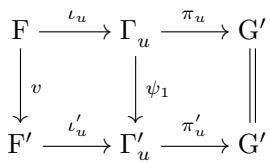
\includegraphics[keepaspectratio]{images/part002_ccea47d6.jpg}}

commutes and \(\varphi_{u}^{\prime}\circ\psi_{1}=\varphi_{v}\circ\varphi_{u}\) . The existence of \(\psi\) follows from Proposition 2 applied to \(\psi_{1}\) . Conversely, if \(\psi^{\prime}\) also has the desired properties, then we have \(\psi^{\prime}\circ\varphi_{v}^{\prime}=\psi_{1}\) by Lemma 2, so \(\psi^{\prime}=\psi\) (Proposition 2).

\subsection{\texorpdfstring{Group Law on the Classes of \(\tau\)-Extensions}{Group Law on the Classes of \textbackslash tau-Extensions}}

Let \(\mathrm{G}\) be a group, \(\mathrm{F}\) be an abelian group, and \(\tau : \mathrm{G} \to \mathrm{Aut}(\mathrm{F})\) be a group homomorphism. We denote by \(\delta : \mathrm{G} \to \mathrm{G} \times \mathrm{G}\) the diagonal mapping \(g \mapsto (g, g)\) and by \(m : \mathrm{F} \times \mathrm{F} \to \mathrm{F}\) the multiplication homomorphism \((f_1, f_2) \mapsto f_1 f_2\) . We denote by \(s : \mathrm{F} \to \mathrm{F}\) the group homomorphism given by \(f \mapsto f^{-1}\) . Let \(\mathcal{E}_1 = (\Gamma_1, \iota_1, \pi_1)\) and \(\mathcal{E}_2 = (\Gamma_2, \iota_2, \pi_2)\) be \(\tau\) -extensions of \(\mathrm{G}\) by \(\mathrm{F}\) . Since we have the relation

\[
m (((\tau \times \tau) \circ \delta) (g) \cdot (f _ {1}, f _ {2})) = \tau (g) \cdot m (f _ {1}, f _ {2})
\]

for every \(g \in G\) and all \(f_{1}, f_{2} \in F\) , the extension \(m_{*}(\delta^{*}(\mathcal{E}_{1} \times \mathcal{E}_{2}))\) is a \(\tau\) -extension; we call it the product of the \(\tau\) -extensions \(E_{1}\) and \(E_{2}\) and denote it by \(E_{1}E_{2}\) . The class of this extension depends only on the classes of the extensions \(E_{1}\) and \(E_{2}\) (VIII, p.~288, Corollary 1 and VIII, p.~291, Corollary 1). So this gives a law of composition on \(\operatorname{Ex}_{\tau}(\mathbf{G}, \mathbf{F})\) .

Remark. --- Let \(\mathcal{E}_{1}=(\Gamma_{1},\iota_{1},\pi_{1})\) and \(\mathcal{E}_{2}=(\Gamma_{2},\iota_{2},\pi_{2})\) be \(\tau\) -extensions of G by F. Let \(\mathcal{E}_{1}\mathcal{E}_{2}=(\Gamma,\iota,\pi)\) be the product of these extensions. Following the example of VIII, p.~289, the construction gives a surjective group homomorphism from the fiber product \(\Gamma_{1}\times_{G}\Gamma_{2}\) to \(\Gamma\) whose kernel is the image of the group homomorphism \(f\mapsto(\iota_{1}(f),\iota_{2}(f)^{-1})\) from F to \(\Gamma_{1}\times_{G}\Gamma_{2}\) .

PROPOSITION 4. --- The product of \(\tau\) -extensions endows the set \(\mathrm{Ex}_{\tau}(\mathrm{G},\mathrm{F})\) with the structure of an abelian group. Its identity element is the class of the semitrivial extension \(\mathcal{I}_{\tau}\) . The inverse of the class of a \(\tau\) -extension \(\mathcal{E}\) is the class of \(s_{*}(\mathcal{E})\) .

The associativity of the law follows from the commutativity of the diagrams

\pandocbounded{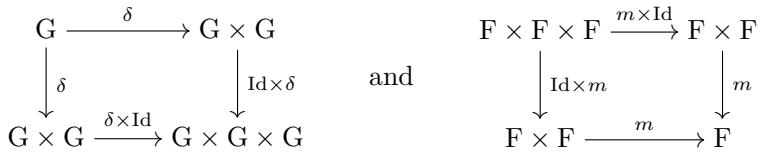
\includegraphics[keepaspectratio]{images/part002_39f17f00.jpg}}

and from Corollary 2 of VIII, p.~288; Corollary 2 of VIII, p.~291; and Proposition 3 of VIII, p.~292.

Let \(\Delta : \mathrm{F} \to \mathrm{F} \times \mathrm{F}\) be the diagonal mapping \(f \mapsto (f, f)\) . Let \(\mathcal{E} = (\Gamma, \iota, \pi)\) be a \(\tau\) -extension. Let \(\widetilde{\Delta}: \Gamma \to \Gamma \times_{\mathrm{G}} \Gamma\) be the group homomorphism given by \(\gamma \mapsto (\gamma, \gamma)\) . The following diagram commutes:

\pandocbounded{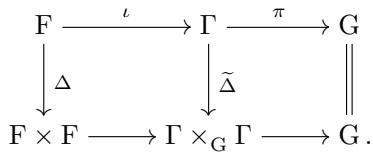
\includegraphics[keepaspectratio]{images/part002_db57599b.jpg}}

By Proposition 2 of VIII, p.~290, it follows that the \((\tau \times \tau) \circ \delta\) -extension \(\delta^{*}(\mathcal{E} \times \mathcal{E})\) is isomorphic to \(\Delta_{*}(\mathcal{E})\) .

Denote by \(c: F \to F\) the constant homomorphism \(f \mapsto 1\) . by Example 1 of VIII, p.~292, the fact that \(\mathcal{I}_{\tau}\) is an identity element for this law of composition follows from the isomorphism from \(\delta^{*}(\mathcal{E} \times \mathcal{E})\) to \(\Delta_{*}(\mathcal{E})\) and the commutative diagram

\pandocbounded{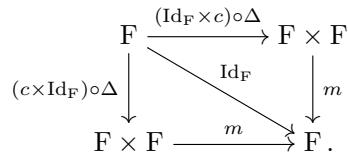
\includegraphics[keepaspectratio]{images/part002_761b87f2.jpg}}

The last assertion follows from the commutative diagram

\[
\begin{array}{c} \mathrm{F} \xrightarrow {(\mathrm{Id} _ {\mathrm{F}} \times s) \circ \Delta} \mathrm{F} \times \mathrm{F} \\ (s \times \mathrm{Id} _ {\mathrm{F}}) \circ \Delta \Biggl \downarrow \qquad \qquad \qquad \qquad \qquad \qquad \qquad \qquad \qquad \qquad \qquad \qquad \qquad \qquad \qquad \qquad \qquad \qquad \qquad \qquad \qquad \qquad \qquad \qquad \qquad \qquad \qquad \qquad \qquad \qquad \qquad \qquad \qquad \qquad \\ \mathrm{F} \times \mathrm{F} \xrightarrow {m} \mathrm{F}. \end{array}
\]

Let \(\mathcal{E}_1 = (\Gamma_1,\iota_1,\pi_1)\) and \(\mathcal{E}_2 = (\Gamma_2,\iota_2,\pi_2)\) be \(\tau\) -extensions. The group isomorphism \(\Gamma_1\times \Gamma_2\to \Gamma_2\times \Gamma_1\) given by \((\gamma_{1},\gamma_{2})\mapsto (\gamma_{2},\gamma_{1})\) restricts to a group isomorphism \(\sigma :\Gamma_1\times_\mathrm{G}\Gamma_2\to \Gamma_2\times_\mathrm{G}\Gamma_1\) . Because of the relations

\[
\sigma (\iota_ {1} (f), \iota_ {2} (f) ^ {- 1}) = (\iota_ {2} (f ^ {- 1}), \iota_ {1} (f ^ {- 1}) ^ {- 1})
\]

for \(f \in F\) , the group homomorphism \(\sigma\) induces, by passing to the quotients, a morphism of \(\tau\) -extensions from \(E_{1}E_{2}\) to \(E_{2}E_{1}\) . So the law of composition is commutative.

PROPOSITION 5. --- a) Let G and G' be groups, and let F be an abelian group. Let \(\tau: \mathrm{G} \to \operatorname{Aut}(\mathrm{F})\) and \(u: \mathrm{G}' \to \mathrm{G}\) be group homomorphisms. The mapping \(u^*: \operatorname{Ex}_{\tau}(\mathrm{G}, \mathrm{F}) \to \operatorname{Ex}_{\tau \circ u}(\mathrm{G}', \mathrm{F})\) is a group homomorphism.

\begin{enumerate}
\def\labelenumi{\alph{enumi})}
\setcounter{enumi}{1}
\tightlist
\item
  Let G be a group, and let F and \(F'\) be abelian groups. Let \(\tau: G \to \text{Aut}(F)\) , \(\tau': G \to \text{Aut}(F')\) , and \(v: F \to F'\) be group homomorphisms such that
\end{enumerate}

\[
\tau^ {\prime} (g) \cdot v (f) = v (\tau (g) \cdot f)
\]

for \(g \in \mathrm{G}\) and \(f \in \mathrm{F}\) . The mapping \(v_{*} : \operatorname{Ex}_{\tau}(\mathrm{G}, \mathrm{F}) \to \operatorname{Ex}_{\tau'}(\mathrm{G}, \mathrm{F}')\) is a group homomorphism.

This follows from the commutativity of the diagrams

\[
\begin{array}{l} \mathrm{G} ^ {\prime} \xrightarrow {\delta} \mathrm{G} ^ {\prime} \times \mathrm{G} ^ {\prime} \\ \Biggl \downarrow_ {u} \qquad \Biggl \downarrow_ {u \times u} \\ \mathrm{G} \xrightarrow {\delta} \mathrm{G} \times \mathrm{G} \end{array} \qquad \text {and} \qquad \begin{array}{l} \mathrm{F} \times \mathrm{F} \xrightarrow {m} \mathrm{F} \\ \Biggl \downarrow_ {v \times v} \qquad \Biggl \downarrow_ {v} \\ \mathrm{F} ^ {\prime} \times \mathrm{F} ^ {\prime} \xrightarrow {m} \mathrm{F} ^ {\prime}. \end{array}
\]

\subsection{Cohomological Description}

Let G be a group, let F be an abelian group, and let \(\tau: G \to \text{Aut}(F)\) be a group homomorphism. For any \(g \in G\) and \(f \in F\) , we also write \(^{g}f\) for \(\tau(g) \cdot f\) . A 2-cocycle of G with values in F is a mapping \(c: G \times G \to F\) such that for every \((g_{1}, g_{2}, g_{3}) \in G \times G \times G\) , we have

\[
{ } ^ { g _ { 1 } } c ( g _ { 2 } , g _ { 3 } ) c ( g _ { 1 } , g _ { 2 } g _ { 3 } ) = c ( g _ { 1 } , g _ { 2 } ) c ( g _ { 1 } g _ { 2 } , g _ { 3 } ) .\tag{7}
\]

Since F is commutative, the set of 2-cocycles is a subgroup of the group of mappings from \(G \times G\) to F; we denote it by \(Z^{2}(G,F)\) . We denote the group of mappings from G to F by \(C^{1}(G,F)\) . For every \(h \in C^{1}(G,F)\) and \((g_{1}, g_{2}) \in G \times G\) , set

\[
(\partial h) (g _ {1}, g _ {2}) = ^ {g _ {1}} h (g _ {2}) h (g _ {1} g _ {2}) ^ {- 1} h (g _ {1}).\tag{8}
\]

A simple calculation shows that the mapping \(\partial h: G \times G \to F\) is a 2-cocycle. The mapping \(\partial: C^{1}(G, F) \to Z^{2}(G, F)\) is a group homomorphism. For any \(h \in C^{1}(G, F)\) , the 2-cocycle \(\partial h\) is called a 2-coboundary. The group

\(Z^{2}(G,F)/\partial(C^{1}(G,F))\) is denoted by \(H^{2}(G,F)\) and is called the second cohomology group of G with coefficients in F.

*The notation above agrees with that of X, §6, n° 8, p.~112 concerning group cohomology.*

Let \(\mathcal{E} = (\Gamma, \iota, \pi)\) be a \(\tau\) -extension. Let \(\sigma\) be a section of the surjective mapping \(\pi\) (Set Theory, II, §3, No.~8, p.~86), that is, a mapping from G to \(\Gamma\) such that \(\pi(\sigma(g)) = g\) for every \(g\) in G. For every \(g_1, g_2 \in G\) , \(\sigma(g_1)\sigma(g_2)\sigma(g_1g_2)^{-1}\) belongs to \(\mathrm{Ker}(\pi)\) , so that there exists a unique mapping \(c_\sigma: G \times G \to F\) such that

\[
\iota (c _ {\sigma} (g _ {1}, g _ {2})) = \sigma (g _ {1}) \sigma (g _ {2}) \sigma (g _ {1} g _ {2}) ^ {- 1}\tag{9}
\]

for all \(g_{1}, g_{2} \in G\) . The mapping \(c_{\sigma}\) is constant with value 1 if and only if \(\sigma\) is a group homomorphism.

PROPOSITION 6. --- The mapping \(c_{\sigma}\) is an element of the group \(Z^{2}(G,F)\) , and its class in the cohomology group \(H^{2}(G,F)\) depends only on the class of the \(\tau\) -extension E.

We say that the mapping \(c_{\sigma}\) is the 2-cocycle associated with \(\sigma\) and that its cohomology class in \(\mathrm{H}^2 (\mathrm{G},\mathrm{F})\) is the cohomology class of the \(\tau\) -extension \(\mathcal{E}\) .

Let us first verify that \(c_{\sigma}\) satisfies the cocycle condition. Let \(g_{1}, g_{2}\) , and \(g_{3}\) be elements of G. Using formula (1) of VIII, p.~285 and (9), we obtain the relations

\[
\begin{array}{r l} & {\iota (g _ {1} c _ {\sigma} (g _ {2}, g _ {3}) c _ {\sigma} (g _ {1}, g _ {2} g _ {3}))} \\ & {\quad = \sigma (g _ {1}) \sigma (g _ {2}) \sigma (g _ {3}) \sigma (g _ {2} g _ {3}) ^ {- 1} \sigma (g _ {1}) ^ {- 1} \sigma (g _ {1}) \sigma (g _ {2} g _ {3}) \sigma (g _ {1} g _ {2} g _ {3}) ^ {- 1}} \\ & {\quad = \sigma (g _ {1}) \sigma (g _ {2}) \sigma (g _ {3}) \sigma (g _ {1} g _ {2} g _ {3}) ^ {- 1}} \end{array}
\]

and

\[
\begin{array}{r l} & {\iota (c _ {\sigma} (g _ {1}, g _ {2}) c _ {\sigma} (g _ {1} g _ {2}, g _ {3}))} \\ & {\qquad = \sigma (g _ {1}) \sigma (g _ {2}) \sigma (g _ {1} g _ {2}) ^ {- 1} \sigma (g _ {1} g _ {2}) \sigma (g _ {3}) \sigma (g _ {1} g _ {2} g _ {3}) ^ {- 1}} \\ & {\qquad = \sigma (g _ {1}) \sigma (g _ {2}) \sigma (g _ {3}) \sigma (g _ {1} g _ {2} g _ {3}) ^ {- 1}.} \end{array}
\]

The mapping \(c_{\sigma}\) is therefore an element of \(\mathbf{Z}^2 (\mathrm{G},\mathrm{F})\) .

Let us now prove that the image of \(c_{\sigma}\) in \(\mathrm{H}^{2}(\mathrm{G},\mathrm{F})\) is independent of the chosen section \(\sigma\) . Let \(\sigma\) and \(\sigma'\) be such sections. For every element g of G, there exists a unique element \(a_{g}\) of F such that \(\sigma'(g) = \iota(a_{g})\sigma(g)\) . Let \(g_{1}\) and \(g_{2}\) be elements of G. Using the definition (9), we obtain the equalities

\[
\begin{array}{r l} & {\iota (c _ {\sigma^ {\prime}} (g _ {1}, g _ {2})) = \sigma^ {\prime} (g _ {1}) \sigma^ {\prime} (g _ {2}) \sigma^ {\prime} (g _ {1} g _ {2}) ^ {- 1}} \\ & {\qquad = \iota (a _ {g _ {1}}) \sigma (g _ {1}) \iota (a _ {g _ {2}}) \sigma (g _ {2}) \sigma (g _ {1} g _ {2}) ^ {- 1} \iota (a _ {g _ {1} g _ {2}}) ^ {- 1}} \\ & {\qquad = \iota (a _ {g _ {1}}) \iota (^ {g _ {1}} a _ {g _ {2}}) \iota (c _ {\sigma} (g _ {1}, g _ {2})) \iota (a _ {g _ {1} g _ {2}}) ^ {- 1}.} \end{array}\tag{10}
\]

Since the group F is commutative, we have the relations

\[
c _ {\sigma^ {\prime}} (g _ {1}, g _ {2}) c _ {\sigma} (g _ {1}, g _ {2}) ^ {- 1} = (^ {g _ {1}} a _ {g _ {2}}) a _ {g _ {1} g _ {2}} ^ {- 1} a _ {g _ {1}} = (\partial a) (g _ {1}, g _ {2}),\tag{11}
\]

as follows from (8). This proves that the classes of \(c_{\sigma'}\) and \(c_{\sigma}\) in \(\mathrm{H}^2(\mathrm{G},\mathrm{F})\) coincide.

Finally, let \(\mathcal{E} = (\Gamma, \iota, \pi)\) and \(\mathcal{E}' = (\Gamma', \iota', \pi')\) be isomorphic \(\tau\) -extensions, let \(u: \mathcal{E} \to \mathcal{E}'\) be a morphism of \(\tau\) -extensions, and let \(\sigma\) be a section of the mapping \(\pi\) . The mapping \(u \circ \sigma\) is a section of the mapping \(\pi'\) , and we have \(c_{\sigma} = c_{u \circ \sigma}\) . The class of \(c_{\sigma}\) in \(\mathrm{H}^2(\mathrm{G}, \mathrm{F})\) therefore depends only on the class of \(\mathcal{E}\) in \(\mathrm{Ex}_{\tau}(\mathrm{G}, \mathrm{F})\) .

We denote by \(\Theta_{\tau}: \operatorname{Ex}_{\tau}(\mathrm{G},\mathrm{F}) \to \mathrm{H}^{2}(\mathrm{G},\mathrm{F})\) , or more simply \(\Theta\) , the mapping that sends the class of a \(\tau\) -extension \((\Gamma,\iota,\pi)\) to the class of the 2-cocycle \(c_{\sigma}\) , where \(\sigma\) is a section of the surjection \(\pi\) .

THEOREM 1. --- The mapping \(\Theta\) is a group isomorphism from \(\operatorname{Ex}_{\tau}(\mathrm{G},\mathrm{F})\) to \(\mathrm{H}^2 (\mathrm{G},\mathrm{F})\) .

Let us first prove that \(\Theta\) is a group homomorphism. Let \(\mathcal{E} = (\Gamma, \iota, \pi)\) and \(\mathcal{E}' = (\Gamma', \iota', \pi')\) be \(\tau\) -extensions, and let \(\sigma\) (resp. \(\sigma'\) ) be a section of the mapping \(\pi\) (resp. \(\pi'\) ). We denote by \(\mathcal{E}\mathcal{E}' = (\Gamma'', \iota'', \pi'')\) the product of the \(\tau\) -extensions E and \(E'\) . We denote by \([\gamma, \gamma']\) the image in \(\Gamma''\) of an element \((\gamma, \gamma')\) of \(\Gamma \times_{G} \Gamma'\) by the surjective homomorphism from the remark of VIII, p.~293. The mapping from G to \(\Gamma''\) that sends an element g to \([\sigma(g), \sigma'(g)]\) is a section \(\sigma''\) of the mapping \(\pi''\) . Let \(g_1\) and \(g_2\) be elements of G. We have the relations

\[
\begin{array}{r l} & {\iota^ {\prime \prime} (c _ {\sigma^ {\prime \prime}} (g _ {1}, g _ {2})) = \sigma^ {\prime \prime} (g _ {1}) \sigma^ {\prime \prime} (g _ {2}) \sigma^ {\prime \prime} (g _ {1} g _ {2}) ^ {- 1}} \\ & {\qquad = [ \iota (c _ {\sigma} (g _ {1}, g _ {2})), \iota^ {\prime} (c _ {\sigma^ {\prime}} (g _ {1}, g _ {2}) ]} \\ & {\qquad = \iota^ {\prime \prime} (c _ {\sigma} (g _ {1}, g _ {2}) c _ {\sigma^ {\prime}} (g _ {1}, g _ {2})).} \end{array}
\]

We therefore have \(c_{\sigma''}(g_1, g_2) = c_\sigma(g_1, g_2)c_{\sigma'}(g_1, g_2)\) .

Let us prove that the mapping \(\Theta\) is injective. Let \(\mathcal{E} = (\Gamma, \iota, \pi)\) be a \(\tau\) -extension, and let \(\sigma\) be a section of the mapping \(\pi\) such that the image of \(c_{\sigma}\) in \(\mathrm{H}^{2}(\mathrm{G}, \mathrm{F})\) is trivial. There exists a mapping \(a : G \to F\) such that

\[
c _ {\sigma} (g _ {1}, g _ {2}) = (^ {g _ {1}} a (g _ {2})) a (g _ {1} g _ {2}) ^ {- 1} a (g _ {1})
\]

for all \(g_{1}, g_{2} \in G\) . We then define \(\sigma' : G \to \Gamma\) by

\[
\sigma^ {\prime} (g) = \iota (a (g) ^ {- 1}) \sigma (g)
\]

for \(g \in G\) . Using (11), we obtain that \(c_{\sigma'}\) is constant with value 1; consequently, \(\sigma'\) is a group homomorphism, which proves that the \(\tau\) -extension E is semitrivial (I, §6, No.~1, p.~67, Proposition 4).

Let us prove that the mapping \(\Theta\) is surjective. Let c be an element of \(Z^{2}(G,F)\) . We endow the set \(\Gamma = F \times G\) with the following law of composition:

\[
(f _ {1}, g _ {1}) (f _ {2}, g _ {2}) = \left(f _ {1} (^ {g _ {1}} f _ {2}) c (g _ {1}, g _ {2}), g _ {1} g _ {2}\right)\tag{12}
\]

for all \(f_{1}, f_{2} \in F\) and \(g_{1}, g_{2} \in G\) . We have the relations

\[
\begin{array}{r l} (f _ {1}, g _ {1}) ((f _ {2}, g _ {2}) (f _ {3}, g _ {3})) & = (f _ {1}, g _ {1}) \big (f _ {2} (^ {g _ {2}} f _ {3}) c (g _ {2}, g _ {3}), g _ {2} g _ {3} \big) \\ & = \big (f _ {1} (^ {g _ {1}} f _ {2}) (^ {g _ {1} g _ {2}} f _ {3}) (^ {g _ {1}} c (g _ {2}, g _ {3})) c (g _ {1}, g _ {2} g _ {3}), g _ {1} g _ {2} g _ {3} \big) \end{array}
\]

and

\[
\begin{array}{c} ((f _ {1}, g _ {1}) (f _ {2}, g _ {2}))   (f _ {3}, g _ {3}) = \big (f _ {1} (^ {g _ {1}} f _ {2}) c (g _ {1}, g _ {2}), g _ {1} g _ {2} \big) (f _ {3}, g _ {3}) \\ = \big (f _ {1} (^ {g _ {1}} f _ {2}) (^ {g _ {1} g _ {2}} f _ {3}) c (g _ {1}, g _ {2}) c (g _ {1} g _ {2}, g _ {3}), g _ {1} g _ {2} g _ {3} \big) \end{array}
\]

for all \(f_{1}, f_{2}, f_{3} \in F\) and \(g_{1}, g_{2}, g_{3} \in G\) . It follows that this law is associative because c is a 2-cocycle. For every \((f, g) \in \Gamma\) , we have

\[
(f, g) (c (e, e) ^ {- 1}, e) = (f (^ {g} c (e, e) ^ {- 1}) c (g, e), g).
\]

Now, it follows from the definition of a 2-cocycle that \(c(g, e) = {}^g c(e, e)\) , from which we deduce that \((f, g)(c(e, e)^{-1}, e) = (f, g)\) . We prove likewise that

\[
(c (e, e) ^ {- 1}, e) (f, g) = (f c (e, e) ^ {- 1} c (e, g), g) = (f, g).
\]

The law of composition defined by (12) therefore has identity element \((c(e,e)^{-1},e)\) , and every element \((f,g)\) of \(\Gamma\) is invertible, with inverse

\[
\left(^ {g ^ {- 1}} (f ^ {- 1} c (e, e) ^ {- 1} c (g, g ^ {- 1}) ^ {- 1}), g ^ {- 1}\right).
\]

So we have endowed \(\Gamma\) with a group structure. Let us denote by \(\iota: F \to G\) the mapping that sends f to \((c(e, e)^{-1}f, e)\) , by \(\pi: \Gamma \to G\) the second projection, and by \(\sigma\) the mapping \(g \mapsto (1, g)\) . The mappings \(\iota\) and \(\pi\) are group homomorphisms, so the triple \(\mathcal{E} = (\Gamma, \iota, \pi)\) is a \(\tau\) -extension, \(\sigma\) is a section of the mapping \(\pi\) , and the associated cocycle \(c_{\sigma}\) is equal to c because

\[
\begin{array}{c} \sigma (g _ {1}) \sigma (g _ {2}) \sigma (g _ {1} g _ {2}) ^ {- 1} = (1, g _ {1}) (1, g _ {2}) (1, g _ {1} g _ {2}) ^ {- 1} = (c (g _ {1}, g _ {2}), g _ {1} g _ {2}) (1, g _ {1} g _ {2}) ^ {- 1} \\ = (c (g _ {1}, g _ {2}) c (e, g _ {1} g _ {2}) ^ {- 1}, e) = (c (e, e) ^ {- 1} c (g _ {1}, g _ {2}), e) \end{array}
\]

for \(g_{1}, g_{2} \in G\) .

Remark. --- Let G be a group, let F and \(F'\) be abelian groups, let \(\tau\) (resp. \(\tau'\) ) be a group homomorphism from G to the automorphism group of F (resp. \(F'\) ), and let \(v : F \to F'\) be a group morphism such that

\[
v (\tau (g) \cdot f) = \tau^ {\prime} (g) \cdot v (f)\tag{13}
\]

for \(g \in G\) and \(f \in F\) . Let \(\alpha\) be an element of \(\operatorname{Ex}_{\tau}(\mathrm{G}, \mathrm{F})\) . If the cocycle c represents \(\Theta(\alpha)\) , then \(v \circ c\) represents \(\Theta(v_{*}(\alpha)) \in \mathrm{H}^{2}(\mathrm{G}, \mathrm{F}')\) .

\subsection{Restriction and Corestriction}

Let G and \(G'\) be groups, F be an abelian group, and \(\tau\) be a homomorphism from G to the automorphism group of F. Let \(u: G' \to G\) be a group homomorphism. We write \(\tau' = \tau \circ u\) .

If \(\psi : \mathrm{G} \times \mathrm{G} \to \mathrm{F}\) is a 2-cocycle of \(\mathrm{G}\) with values in \(\mathrm{F}\) , then the mapping \(\psi \circ (u \times u)\) from \(\mathrm{G}' \times \mathrm{G}'\) to \(\mathrm{F}\) given by \((g_1, g_2) \mapsto \psi(u(g_1), u(g_2))\) is a 2-cocycle of \(\mathrm{G}'\) with values in \(\mathrm{F}\) , and the mapping \(\psi \mapsto \psi \circ (u \times u)\) from \(\mathrm{Z}^2(\mathrm{G}, \mathrm{F})\) to \(\mathrm{Z}^2(\mathrm{G}', \mathrm{F})\) induces a group homomorphism \(u^*: \mathrm{H}^2(\mathrm{G}, \mathrm{F}) \to \mathrm{H}^2(\mathrm{G}', \mathrm{F})\) . For any \(\lambda \in \mathrm{H}^2(\mathrm{G}, \mathrm{F})\) , the element \(u^*(\lambda)\) is called the inverse image of \(\lambda\) by \(u\) . When \(\mathrm{G}'\) is a subgroup of \(\mathrm{G}\) and \(u: \mathrm{G}' \to \mathrm{G}\) is the canonical injection, the homomorphism \(u^*\) is called the restriction homomorphism from \(\mathrm{G}\) to \(\mathrm{G}'\) ; we denote it by \(\operatorname{Res}_{\mathrm{G}'}^{\mathrm{G}}\) . When \(\mathrm{G}\) is a quotient of \(\mathrm{G}'\) and \(u: \mathrm{G}' \to \mathrm{G}\) is the canonical surjection, the homomorphism \(u^*\) is called the inflation homomorphism from \(\mathrm{G}\) to \(\mathrm{G}'\) .

PROPOSITION 7. --- In the notation from above, the following diagram commutes:

\[
\begin{array}{c} \operatorname{Ex} _ {\tau} (\mathrm{G}, \mathrm{F}) \xrightarrow {u ^ {*}} \operatorname{Ex} _ {\tau} (\mathrm{G} ^ {\prime}, \mathrm{F}) \\ \Biggl \downarrow \Theta_ {\tau} \qquad \qquad \qquad \Biggl \downarrow \Theta_ {\tau^ {\prime}} \\ \operatorname{H} ^ {2} (\mathrm{G}, \mathrm{F}) \xrightarrow {u ^ {*}} \operatorname{H} ^ {2} (\mathrm{G} ^ {\prime}, \mathrm{F})  . \end{array}
\]

Let H be a subgroup of G of finite index. Let s be a section of the canonical surjection from G to \(H\backslash G\). We denote by \((g,x)\mapsto x\cdot g\) the right action of G on \(H\backslash G\) induced by the right action of G on itself by multiplication. Note that for every \(x\in H\backslash G\) and \(g\in G\) , the element \(s(x)gs(x\cdot g)^{-1}\) belongs to H. For any mapping \(c: \mathrm{H} \times \mathrm{H} \to \mathrm{F}\) , we can therefore define a mapping \(\widetilde{c}_s: \mathrm{G} \times \mathrm{G} \to \mathrm{F}\) by the relation

\[
\widetilde {c} _ {s} (g _ {1}, g _ {2}) = \prod_ {x \in \mathrm{H} \backslash \mathrm{G}} ^ {s (x) ^ {- 1}} c \bigl (s (x) g _ {1} s (x \cdot g _ {1}) ^ {- 1}, s (x \cdot g _ {1}) g _ {2} s (x \cdot g _ {1} g _ {2}) ^ {- 1} \bigr)
\]

for \(g_{1}, g_{2} \in G\) . The mapping \(c \mapsto \widetilde{c}_{s}\) is a group homomorphism from \(F^{H \times H}\) to \(F^{G \times G}\) .

Lemma 4. --- If \(c: \mathrm{H} \times \mathrm{H} \to \mathrm{F}\) is a 2-cocycle of H with values in F, then \(\widetilde{c}_s\) is a 2-cocycle of G with values in F.

Let \(g_1, g_2\) , and \(g_3\) be elements of G. For every \(i \in \{1, 2, 3\}\) , we define a mapping \(h_i: \mathrm{H} \backslash \mathrm{G} \to \mathrm{H}\) by the relation

\[
h _ {i} (x) = s \left(x \cdot g _ {1} \dots g _ {i - 1}\right) g _ {i} s \left(x \cdot g _ {1} \dots g _ {i}\right) ^ {- 1}
\]

for \(x\in \mathrm{H}\backslash \mathrm{G}\) . Note that

\[
\begin{array}{l} {h _ {1} (x) h _ {2} (x) = s (x) g _ {1} g _ {2} s (x \cdot g _ {1} g _ {2}) ^ {- 1}} \\ {h _ {2} (x) h _ {3} (x) = s (x \cdot g _ {1}) g _ {2} g _ {3} s (x \cdot g _ {1} g _ {2} g _ {3}) ^ {- 1}} \end{array}
\]

for \(x \in \mathrm{H} \backslash \mathrm{G}\) . We then have the relations

\[
\begin{array}{r l} & ^ {g _ {1}} \widetilde {c} _ {s} (g _ {2}, g _ {3}) \widetilde {c} _ {s} (g _ {1} g _ {2}, g _ {3}) ^ {- 1} \widetilde {c} _ {s} (g _ {1}, g _ {2} g _ {3}) \widetilde {c} _ {s} (g _ {1}, g _ {2}) ^ {- 1} \\ & \quad = \prod_ {x \in \mathrm{H} \backslash \mathrm{G}} ^ {g _ {1} s (x) ^ {- 1}} c \big (s (x) g _ {2} s (x \cdot g _ {2}) ^ {- 1}, s (x \cdot g _ {2}) g _ {3} s (x \cdot g _ {2} g _ {3}) ^ {- 1} \big) \\ & \qquad \times \prod_ {x \in \mathrm{H} \backslash \mathrm{G}} ^ {s (x) ^ {- 1}} \Big (c (h _ {1} (x) h _ {2} (x), h _ {3} (x)) ^ {- 1} \\ & \qquad \qquad \qquad \qquad \times c (h _ {1} (x), h _ {2} (x) h _ {3} (x))   c (h _ {1} (x), h _ {2} (x)) ^ {- 1} \Big) \\ & = \prod_ {x \in \mathrm{H} \backslash \mathrm{G}} ^ {s (x \cdot g _ {1} ^ {- 1}) ^ {- 1} h _ {1} (x \cdot g _ {1} ^ {- 1})} c (h _ {2} (x \cdot g _ {1} ^ {- 1}), h _ {3} (x \cdot g _ {1} ^ {- 1})) \\ & \qquad \times \prod_ {x \in \mathrm{H} \backslash \mathrm{G}} ^ {s (x) ^ {- 1} h _ {1} (x)} c (h _ {2} (x), h _ {3} (x)) ^ {- 1} \\ & = 1, \end{array}
\]

where the second equality follows from the fact that c is a 2-cocycle.

Lemma 5. --- If \(c\) is a 2-coboundary, then so is \(\widetilde{c}_s\) .

Let \(t: \mathrm{H} \to \mathrm{F}\) be a mapping such that \(c = \partial t\) . Let \(\widetilde{t}_s: \mathrm{G} \to \mathrm{F}\) be the mapping defined by

\[
\widetilde {t} _ {s} (g) = \prod_ {x \in \mathrm{H} \backslash \mathrm{G}} ^ {s (x) ^ {- 1}} t (s (x) g s (x \cdot g) ^ {- 1})
\]

for \(g \in G\) . It suffices to prove that \(\widetilde{c}_{s} = \partial\widetilde{t}_{s}\) , which follows from the relations

\[
\begin{array}{l} \widetilde {c} _ {s} (g _ {1}, g _ {2}) = \prod_ {x \in \mathrm{H} \backslash \mathrm{G}} ^ {s (x) ^ {- 1} s (x) g _ {1} s (x \cdot g _ {1}) ^ {- 1}} t (s (x \cdot g _ {1}) g _ {2} s (x \cdot g _ {1} g _ {2}) ^ {- 1}) \\ \qquad \times \prod_ {x \in \mathrm{H} \backslash \mathrm{G}} ^ {s (x) ^ {- 1}} \big (t (s (x) g _ {1} g _ {2} s (x \cdot g _ {1} g _ {2}) ^ {- 1}) ^ {- 1} t (s (x) g _ {1} s (x \cdot g _ {1}) ^ {- 1}) \big) \\ = \partial \widetilde {t} _ {s} (g _ {1}, g _ {2}) \end{array}
\]

for \(g_{1}, g_{2} \in G\) .

Lemma 6. --- Let c be a 2-cocycle of H with values in F. The image of \(\widetilde{c}_{s}\) in the group \(\mathrm{H}^{2}(\mathrm{G},\mathrm{F})\) does not depend on the choice of the section s.

Let \(s'\) be a section of the canonical surjection from G to \(H\backslash G\). Let \(h: \mathrm{H} \backslash \mathrm{G} \to \mathrm{H}\) be the mapping characterized by the relation

\[
s ^ {\prime} (x) = h (x) s (x)
\]

for \(x \in H \backslash G\) . The 2-cocycle \(\widetilde{c}_{s'}\) is then given by the relations

\[
\begin{array}{l} \widetilde {c} _ {s ^ {\prime}} (g _ {1}, g _ {2}) \\ = \prod_ {x \in \mathrm{H} \backslash \mathrm{G}} ^ {s (x) ^ {- 1} h (x) ^ {- 1}} c \big (h (x) s (x) g _ {1} s ^ {\prime} (x \cdot g _ {1}) ^ {- 1}, s ^ {\prime} (x \cdot g _ {1}) g _ {2} s ^ {\prime} (x \cdot g _ {1} g _ {2}) ^ {- 1} \big) \\ = \prod_ {x \in \mathrm{H} \backslash \mathrm{G}} ^ {s (x) ^ {- 1}} c \big (s (x) g _ {1} s (x \cdot g _ {1}) ^ {- 1} h (x \cdot g _ {1}) ^ {- 1}, h (x \cdot g _ {1}) s (x \cdot g _ {1}) g _ {2} s ^ {\prime} (x \cdot g _ {1} g _ {2}) ^ {- 1} \big) \\ \qquad \times \prod_ {x \in \mathrm{H} \backslash \mathrm{G}} ^ {s (x) ^ {- 1}} \Big (c \big (h (x) ^ {- 1}, s ^ {\prime} (x) g _ {1} g _ {2} s ^ {\prime} (x \cdot g _ {1} g _ {2}) ^ {- 1} \big) ^ {- 1} \\ \qquad \qquad \qquad \qquad \qquad \qquad \qquad \qquad \qquad \qquad \qquad \qquad \qquad \qquad \qquad \qquad \qquad \qquad \qquad \qquad \qquad \qquad \qquad \qquad \qquad \qquad \qquad \qquad \qquad \qquad \qquad \qquad \qquad \qquad \\ = \prod_ {x \in \mathrm{H} \backslash \mathrm{G}} ^ {g _ {1} s (x \cdot g _ {1}) ^ {- 1}} c \big (h (x \cdot g _ {1}) ^ {- 1}, h (x \cdot g _ {1}) s (x \cdot g _ {1}) g _ {2} s ^ {\prime} (x \cdot g _ {1} g _ {2}) ^ {- 1} \big) \\ \qquad \times \prod_ {x \in \mathrm{H} \backslash \mathrm{G}} ^ {s (x) ^ - 1} c \big (s (x) g _ {1} s (x \cdot g _ {1}) ^ {- 1}, s (x \cdot g _ {1}) g _ {2} s ^ {\prime} (x \cdot g _ {1} g _ {2}) ^ {- 1} \big) \\ \qquad \times \prod_ {x \in \mathrm{H} \backslash \mathrm{G}} ^ {s (x) ^ {- 1}} c \big (s (x) g _ {1} s (x \cdot g _ {1}) ^ {- 1}, h (x \cdot g _ {1}) ^ {- 1} \big) ^ {- 1} \\ \qquad \times \prod_ {x \in \mathrm{H} \backslash \mathrm{G}} ^ {s (x) ^ {- 1}} \Big (c \big (h (x) ^ {- 1}, s ^ {\prime} (x) g _ {1} g _ {2} s ^ {\prime} (x \cdot g _ {1} g _ {2}) ^ {- 1} \big) ^ {{- 1}} \\ \qquad \qquad \qquad \qquad \qquad \qquad \qquad \qquad \qquad \qquad \qquad \qquad \times c (h (x) ^ {- 1}, s ^ {\prime} (x) g _ {1} s ^ {\prime} (x \cdot g _ {1}) ^ {- 1})   {\Big)} \end{array}
\]

\[
\begin{array}{l} = \prod_ {x \in \mathrm{H} \backslash \mathrm{G}} ^ {s (x) ^ {- 1}} c \big (s (x) g _ {1} s (x \cdot g _ {1}) ^ {- 1}, s (x \cdot g _ {1}) g _ {2} s ^ {\prime} (x \cdot g _ {1} g _ {2}) ^ {- 1} \big) \\ \qquad \times \prod_ {x \in \mathrm{H} \backslash \mathrm{G}} ^ {s (x) ^ {- 1}} c \big (s (x) g _ {1} s (x \cdot g _ {1}) ^ {- 1}, h (x \cdot g _ {1}) ^ {- 1} \big) ^ {- 1} \\ \qquad \times \prod_ {x \in \mathrm{H} \backslash \mathrm{G}} ^ {g _ {1} s (x) ^ {- 1}} c \big (h (x) ^ {- 1}, h (x) s (x) g _ {2} s ^ {\prime} (x \cdot g _ {2}) ^ {- 1} \big) \\ \qquad \times \prod_ {x \in \mathrm{H} \backslash \mathrm{G}} ^ {s (x) ^ {- 1}} \Big (c \big (h (x) ^ {- 1}, s ^ {\prime} (x) g _ {1} g _ {2} s ^ {\prime} (x \cdot g _ {1} g _ {2}) ^ {- 1} \big) ^ {- 1} \\ \qquad \qquad \qquad \qquad \qquad \qquad \qquad \qquad \qquad \qquad \qquad \qquad \qquad \qquad \qquad \qquad \qquad \qquad \times c \big (h (x) ^ {- 1}, s ^ {\prime} (x) g _ {1} s ^ {\prime} (x \cdot g _ {1}) ^ {- 1} \big) \Big) \end{array}
\]

for all \(g_1, g_2 \in \mathbf{G}\) . The first equality comes from the cocycle relation (VIII, p.~295, formula (7)) applied to the elements

\[
h (x) ^ {- 1}, \quad h (x) s (x) g _ {1} s ^ {\prime} (x \cdot g _ {1}) ^ {- 1}, \quad \mathrm{and} \quad s ^ {\prime} (x \cdot g _ {1}) g _ {2} s ^ {\prime} (x \cdot g _ {1} g _ {2}) ^ {- 1};
\]

the second is obtained by applying the cocycle relation to the elements

\[
s (x) g _ {1} s \left(x \cdot g _ {1}\right) ^ {- 1}, \quad h \left(x \cdot g _ {1}\right) ^ {- 1}, \quad \text { and } \quad h \left(x \cdot g _ {1}\right) s \left(x \cdot g _ {1}\right) g _ {2} s ^ {\prime} \left(x \cdot g _ {1} g _ {2}\right) ^ {- 1};
\]

and the last simply uses the fact that the mapping \(x \mapsto x \cdot g_{1}\) is a permutation of \(H\backslash G\).

The last two lines of the obtained expression correspond to a 2-coboundary. We find that \(\widetilde{c}_{s'}\) has the same class in \(\mathrm{H}^2 (\mathrm{G},\mathrm{F})\) as the cocycle whose value in \((g_{1},g_{2})\in \mathrm{G}^{2}\) is given by the expression

\[
\begin{array}{l} \prod_ {x \in \mathrm{H} \backslash \mathrm{G}} ^ {s (x) ^ {- 1}} c \big (s (x) g _ {1} s (x \cdot g _ {1}) ^ {- 1}, s (x \cdot g _ {1}) g _ {2} s (x \cdot g _ {1} g _ {2}) ^ {- 1} h (x \cdot g _ {1} g _ {2}) ^ {- 1} \big) \\ \qquad \qquad \qquad \times \prod_ {x \in \mathrm{H} \backslash \mathrm{G}} ^ {s (x) ^ {- 1}} c \big (s (x) g _ {1} s (x \cdot g _ {1}) ^ {- 1}, h (x \cdot g _ {1}) ^ {- 1} \big) ^ {- 1} \\ = \prod_ {x \in \mathrm{H} \backslash \mathrm{G}} ^ {g _ {1} s (x \cdot g _ {1}) ^ {- 1}} c \big (s (x \cdot g _ {1}) g _ {2} s (x \cdot g _ {1} g _ {2}) ^ {- 1}, h (x \cdot g _ {1} g _ {2}) ^ {- 1} \big) ^ {- 1} \\ \qquad \qquad \times \prod_ {x \in \mathrm{H} \backslash \mathrm{G}} ^ {s (x) ^ {- 1}} c \big (s (x) g _ {1} s (x \cdot g _ {1}) ^ {- 1}, s (x \cdot g _ {1}) g _ {2} s (x \cdot g _ {1} g _ {2}) ^ {- 1} \big) \\ \qquad \qquad \times \prod_ {x \in \mathrm{H} \backslash \mathrm{G}} ^ {s (x) ^ {- 1}} \Big (c \big (s (x) g _ {1} g _ {2} s (x \cdot g _ {1} g _ {2}) ^ {- 1}, h (x \cdot g _ {1} g _ {2}) ^ {- 1} \big) \\ \qquad \qquad \qquad \times c \big (s (x) g _ {1} s (x \cdot g _ {1}) ^ {- 1}, h (x \cdot g _ {1}) ^ {- 1} \big) ^ {- 1} \Big) \end{array}
\]

\[
\begin{array}{l} = \prod_ {x \in \mathrm{H} \backslash \mathrm{G}} ^ {s (x) ^ {- 1}} c \big (s (x) g _ {1} s (x \cdot g _ {1}) ^ {- 1}, s (x \cdot g _ {1}) g _ {2} s (x \cdot g _ {1} g _ {2}) ^ {- 1} \big) \\ \quad \times \prod_ {x \in \mathrm{H} \backslash \mathrm{G}} ^ {g _ {1} s (x) ^ {- 1}} c \big (s (x) g _ {2} s (x \cdot g _ {2}) ^ {- 1}, h (x \cdot g _ {2}) ^ {- 1} \big) ^ {- 1} \\ \quad \times \prod_ {x \in \mathrm{H} \backslash \mathrm{G}} ^ {s (x) ^ {- 1}} \Big (c \big (s (x) g _ {1} g _ {2} s (x \cdot g _ {1} g _ {2}) ^ {- 1}, h (x \cdot g _ {1} g _ {2}) ^ {- 1} \big) \\ \qquad \qquad \qquad \qquad \qquad \qquad \qquad \qquad \qquad \qquad \qquad \qquad \qquad \times c \big (s (x) g _ {1} s (x \cdot g _ {1}) ^ {- 1}, h (x \cdot g _ {1}) ^ {- 1} \big) ^ {- 1} \Big), \end{array}
\]

where the first equality follows from the cocycle relation applied to the elements

\[
s (x) g _ {1} s (x \cdot g _ {1}) ^ {- 1}, \quad s (x \cdot g _ {1}) g _ {2} s (x \cdot g _ {1} g _ {2}) ^ {- 1}, \quad \text { and } \quad h (x \cdot g _ {1} g _ {2}) ^ {- 1}.
\]

The last two lines of the obtained expression correspond to a 2-coboundary. We find that the class of \(\widetilde{c}_{s'}\) coincides with that of \(\widetilde{c}_s\) .

We have constructed a homomorphism from the group \(\mathrm{H}^{2}(\mathrm{H},\mathrm{F})\) to the group \(\mathrm{H}^{2}(\mathrm{G},\mathrm{F})\) , which we call the corestriction homomorphism from H to G and denote by \(Cor_{H}^{G}\) .

PROPOSITION 8. --- Let H be a subgroup of G of finite index. The endomorphism \(Cor_{H}^{G} \circ Res_{H}^{G}\) of the group \(H^{2}(G, F)\) coincides with multiplication by the index \((G : H)\) .

Let \(\alpha\) be an element of \(\mathrm{H}^2 (\mathrm{G},\mathrm{F})\) , and let \(c\) be an element of \(\mathrm{Z}^2 (\mathrm{G},\mathrm{F})\) representing \(\alpha\) . The element \(\mathrm{Cor}_{\mathrm{H}}^{\mathrm{G}}\circ \mathrm{Res}_{\mathrm{H}}^{\mathrm{G}}(\alpha)\) is the class of the cocycle whose value in \((g_{1},g_{2})\in \mathrm{G}^{2}\) is given by the expression

\[
\begin{array}{l} \prod_ {x \in \mathrm{H} \backslash \mathrm{G}} ^ {s (x) ^ {- 1}} c (s (x) g _ {1} s (x \cdot g _ {1}) ^ {- 1}, s (x \cdot g _ {1}) g _ {2} s (x \cdot g _ {1} g _ {2}) ^ {- 1}) \\ = \prod_ {x \in \mathrm{H} \backslash \mathrm{G}} c (g _ {1} s (x \cdot g _ {1}) ^ {- 1}, s (x \cdot g _ {1}) g _ {2} s (x \cdot g _ {1} g _ {2}) ^ {- 1}) \\ \quad \times \prod_ {x \in \mathrm{H} \backslash \mathrm{G}} \big (c (s (x) ^ {- 1}, s (x) g _ {1} g _ {2} s (x \cdot g _ {1} g _ {2}) ^ {- 1}) ^ {- 1} c (s (x) ^ {- 1}, s (x) g _ {1} s (x \cdot g _ {1}) ^ {- 1}) \big) \\ = \prod_ {x \in \mathrm{H} \backslash \mathrm{G}} ^ {g _ {1}} c (s (x \cdot g _ {1}) ^ {- 1}, s (x \cdot g _ {1}) g _ {2} s (x \cdot g _ {1} g _ {2}) ^ {- 1}) \\ \quad \times \prod_ {x \in \mathrm{H} \backslash \mathrm{G}} c (g _ {1}, g _ {2} s (x \cdot g _ {1} g _ {2}) ^ {- 1}) c (g _ {1}, s (x \cdot g _ {1}) ^ {- 1}) ^ {- 1} \\ \quad \times \prod_ {x \in \mathrm{H} \backslash \mathrm{G}} \big (c (s (x) ^ {- 1}, s (x) g _ {1} g _ {2} s (x \cdot g _ {1} g _ {2}) ^ {- 1}) ^ {- 1} c (s (x) ^ {- 1}, s (x) g _ {1} s (x \cdot g _ {1}) ^ {- 1}) \big) \end{array}
\]

\[
\begin{array}{l} = \prod_ {x \in \mathrm{H} \backslash \mathrm{G}} c (g _ {1}, g _ {2} s (x \cdot g _ {1} g _ {2}) ^ {- 1}) c (g _ {1}, s (x \cdot g _ {1}) ^ {- 1}) ^ {- 1} \\ \times \prod_ {x \in \mathrm{H} \backslash \mathrm{G}} ^ {g _ {1}} c (s (x) ^ {- 1}, s (x) g _ {2} s (x g _ {2}) ^ {- 1}) \\ \times \prod_ {x \in \mathrm{H} \backslash \mathrm{G}} \left(c (s (x) ^ {- 1}, s (x) g _ {1} g _ {2} s (x \cdot g _ {1} g _ {2}) ^ {- 1}) ^ {- 1} c (s (x) ^ {- 1}, s (x) g _ {1} s (x \cdot g _ {1}) ^ {- 1})\right). \end{array}
\]

The first equality comes from the cocycle relation (VIII, p.~295, formula (7)) applied to the elements

\[
s (x) ^ {- 1}, \quad s (x) g _ {1} s (x \cdot g _ {1}) ^ {- 1}, \quad \mathrm{and} \quad s (x \cdot g _ {1}) g _ {2} s (x \cdot g _ {1} g _ {2}) ^ {- 1};
\]

the second is obtained by applying the cocycle relation to the elements

\[
g _ {1}, \quad s (x \cdot g _ {1}) ^ {- 1}, \quad \mathrm{and} \quad s (x \cdot g _ {1}) g _ {2} s (x \cdot g _ {1} g _ {2}) ^ {- 1}.
\]

By removing a coboundary, we obtain that \(\mathrm{Cor}_{\mathrm{H}}^{\mathrm{G}} \circ \mathrm{Res}_{\mathrm{H}}^{\mathrm{G}}(\alpha)\) is the class of the cocycle whose value in \((g_{1}, g_{2}) \in \mathrm{G}^{2}\) is given by the expression

\[
\begin{array}{l} \prod_ {x \in \mathrm{H} \backslash \mathrm{G}} c (g _ {1}, g _ {2} s (x \cdot g _ {1} g _ {2}) ^ {- 1}) c (g _ {1}, s (x \cdot g _ {1}) ^ {- 1}) ^ {- 1} \\ = \prod_ {x \in \mathrm{H} \backslash \mathrm{G}} ^ {g _ {1}} c (g _ {2}, s (x \cdot g _ {1} g _ {2}) ^ {- 1}) ^ {- 1} c (g _ {1} g _ {2}, s (x \cdot g _ {1} g _ {2}) ^ {- 1}) c (g _ {1}, g _ {2}) \\ \times \prod_ {x \in \mathrm{H} \backslash \mathrm{G}} c (g _ {1}, s (x \cdot g _ {1}) ^ {- 1}) ^ {- 1} \\ = \prod_ {x \in \mathrm{H} \backslash \mathrm{G}} ^ {g _ {1}} c (g _ {2}, s (x \cdot g _ {2}) ^ {- 1}) ^ {- 1} c (g _ {1} g _ {2}, s (x \cdot g _ {1} g _ {2}) ^ {- 1}) c (g _ {1}, s (x \cdot g _ {1}) ^ {- 1}) ^ {- 1} \\ \times c (g _ {1}, g _ {2}) ^ {\text {(G:H)}}, \end{array}
\]

which proves the result.

\subsection{Galois Algebras}

Let K be a commutative field. If E is a K-algebra, then we denote its automorphism group by \(\operatorname{Aut}_{\mathrm{K}}(\mathrm{E})\) . If E is a Galois extension of the field K, then the group \(\operatorname{Aut}_{\mathrm{K}}(\mathrm{E})\) is simply the Galois group \(\operatorname{Gal}(\mathrm{E}/\mathrm{K})\) (V, §10, No.~2, p.~58).

Let G be a group. A \((K,G)\) -algebra is a K-algebra E endowed with a group homomorphism \(\lambda:G\to\operatorname{Aut}_{K}(E)\) . The homomorphism \(\lambda\) then endows E with the structure of a group with operators in G as well as the structure of a left K{[}G{]}-module with external law given by

\[
\Bigl (\sum_ {g \in \mathrm{G}} \mu_ {g} g \Bigr) x = \sum_ {g \in \mathrm{G}} \mu_ {g} \lambda (g). x\tag{14}
\]

for every \(x \in \mathrm{L}\) and every element \((\mu_g)_{g \in \mathrm{G}}\) of \(\mathrm{K}[\mathrm{G}]\) . A morphism of \((\mathrm{K}, \mathrm{G})\) -algebras is a morphism of algebras that is also a morphism of groups with operators.

For every family \((\mathrm{E}_{i})_{i\in\mathrm{I}}\) of \((\mathrm{K},\mathrm{G})\) -algebras, the product K-algebra \(\prod_{i\in I}E_{i}\) endowed with its structure of a product group with operators is a \((\mathrm{K},\mathrm{G})\) -algebra.

If \(\mathrm{E}\) is a (K, G)-algebra, then the set \(\mathrm{E}^{\mathrm{G}}\) of elements of \(\mathrm{E}\) invariant under \(\mathrm{G}\) is a subalgebra of \(\mathrm{E}\) .

Let E be a (K, G)-algebra, where G acts by \(\lambda: G \to \operatorname{Aut}_{\mathrm{K}}(\mathrm{E})\) . If \(K'\) is an extension of K, then for any \(g \in G\) , let \(\lambda'(g)\) be the automorphism \(\operatorname{Id}_{\mathrm{K}'} \otimes \lambda(g)\) of the \(K'\) -algebra \(\operatorname{L}_{(\mathrm{K}')}\) . Then \(\lambda': g \mapsto \lambda'(g)\) endows \(\operatorname{L}_{(\mathrm{K}')}\) with the structure of a \((\mathrm{K}', \mathrm{G})\) -algebra.

Given a group H and H-sets X and Y, we denote by \(\mathcal{F}_{\mathrm{H}}(\mathrm{X},\mathrm{Y})\) the set of morphisms of H-sets from X to Y. It is the set of mappings \(f:X\to Y\) such that \(f(hx)=hf(x)\) for every \(h\in H\) and \(x\in X\) .

Let G be a group with identity element e, let H be a subgroup of G, and let E be a (K,H)-algebra. The (K,G)-algebra deduced from E by coinduction from H to G, denoted by \(\mathrm{Coind}_{\mathrm{H}}^{\mathrm{G}}(\mathrm{E})\) , is the K-algebra \(\mathcal{F}_{\mathrm{H}}(\mathrm{G},\mathrm{E})\) endowed with the action of G given by the homomorphism \(\lambda\) from G to \(\mathrm{Aut}_{\mathrm{K}}(\mathrm{Coind}_{\mathrm{H}}^{\mathrm{G}}(\mathrm{E}))\) defined by

\[
(\lambda (g) \cdot f) (g ^ {\prime}) = f (g ^ {\prime} g)\tag{15}
\]

for \(f \in \text{Coind}_{\text{H}}^{\text{G}}(\text{E})\) and \(g, g' \in G\) .

Lemma 7. --- a) Let S be a subset of G such that every element of G can be written uniquely as hs with \(h \in H\) and \(s \in S\) . Then the mapping that sends f to \((f(s))_{s \in S}\) is an isomorphism from the K-algebra \(\operatorname{Coind}_{\mathrm{H}}^{\mathrm{G}}(\mathrm{E})\) to the K-algebra \(\mathcal{F}(\mathrm{S}, \mathrm{E})\) of mappings from S to E.

\begin{enumerate}
\def\labelenumi{\alph{enumi})}
\setcounter{enumi}{1}
\tightlist
\item
  The algebra \(\operatorname{Coind}_{\mathrm{H}}^{\mathrm{G}}(\mathrm{E})\) has finite degree over K if and only if E has finite degree over K and the index of H in G is finite. In this case, we have the formula
\end{enumerate}

\[
[ \mathrm{Coind} _ {\mathrm{H}} ^ {\mathrm{G}} (\mathrm{E}): \mathrm{K} ] = (\mathrm{G}: \mathrm{H}) [ \mathrm{E}: \mathrm{K} ].
\]

\begin{enumerate}
\def\labelenumi{\alph{enumi})}
\setcounter{enumi}{2}
\tightlist
\item
  Let \(E^{H}\) be the algebra of invariants of the group H in E and \(\operatorname{Coind}_{\mathrm{H}}^{\mathrm{G}}(\mathrm{E})^{\mathrm{G}}\) that of the group G in \(\operatorname{Coind}_{\mathrm{H}}^{\mathrm{G}}(\mathrm{E})\) . The mapping \(f \mapsto f(e)\)
\end{enumerate}

from \(\mathrm{Coind}_{\mathrm{H}}^{\mathrm{G}}(\mathrm{E})\) to E restricts to an algebra isomorphism from \(\mathrm{Coind}_{\mathrm{H}}^{\mathrm{G}}(\mathrm{E})^{\mathrm{G}}\) to \(\mathrm{E}^{\mathrm{H}}\) .

Assertion a) follows from the definitions and implies b). By (15), a mapping from G to E is an element of \(\mathrm{Coind}_{\mathrm{H}}^{\mathrm{G}}(\mathrm{E})\) invariant under G if and only if it is constant with value an element of E invariant under H.

Remark 1. --- Let G be a group, H a subgroup of G, and N a subgroup of H. Let E be a (K,N)-algebra. Let \(\alpha\) be an element of \(\mathcal{F}_{\mathrm{H}}(\mathrm{G},\mathcal{F}_{\mathrm{N}}(\mathrm{H},\mathrm{E}))\) . We have the relation

\[
\alpha (g) (n h) = n (\alpha (g) (h))\tag{16}
\]

for every \(g \in \mathbf{G}\) , \(h \in \mathbf{H}\) , and \(n \in \mathbf{N}\) and the relations

\[
\alpha (h g) (h ^ {\prime}) = (h \alpha (g)) (h ^ {\prime}) = \alpha (g) (h ^ {\prime} h)\tag{17}
\]

for all \(h, h' \in H\) and every \(g \in G\) . Consequently, \(\alpha(ng)(e) = \alpha(g)(n) = n(\alpha(g)(e))\) for every \(g \in G\) and \(n \in N\) . We can therefore consider the mapping

\[
\psi : \mathcal {F} _ {\mathrm{H}} (\mathrm{G}, \mathcal {F} _ {\mathrm{N}} (\mathrm{H}, \mathrm{E})) \to \mathcal {F} _ {\mathrm{N}} (\mathrm{G}, \mathrm{E})
\]

defined by the relation \(\psi(\alpha)(g)=\alpha(g)(e)\) for \(\alpha\) in \(\mathcal{F}_{\mathrm{H}}(\mathrm{G},\mathcal{F}_{\mathrm{N}}(\mathrm{H},\mathrm{E}))\) and g in G. The mapping \(\psi\) is an algebra isomorphism from \(\operatorname{Coind}_{\mathrm{H}}^{\mathrm{G}}(\operatorname{Coind}_{\mathrm{N}}^{\mathrm{H}}(\operatorname{E}))\) to \(\operatorname{Coind}_{\mathrm{N}}^{\mathrm{G}}(\operatorname{E})\) whose inverse sends an element \(\beta\) from \(\mathcal{F}_{\mathrm{N}}(\mathrm{G},\mathrm{E})\) to the mapping \(\alpha\) defined by the relation \(\alpha(g)(h)=\beta(hg)\) for \(g\in G\) and \(h\in H\) .

We now suppose given a finite group G and a reduced (V, §6, No.~6, p.~32) commutative K-algebra L of finite degree endowed with an action of G given by a homomorphism \(\lambda\) from G to \(\mathrm{Aut}_{\mathrm{K}}(\mathrm{L})\) . For \(x \in \mathrm{L}\) and \(g \in \mathrm{G}\) , we denote by \(g \cdot x\) the transform of \(x\) under the automorphism \(\lambda(g)\) of L. Let \(\mathcal{S}\) be the set of maximal ideals of L; we denote by \(g \cdot \mathfrak{m}\) the transform of an element \(\mathfrak{m}\) of \(\mathcal{S}\) under the automorphism \(\lambda(g)\) of L. It is an element of \(\mathcal{S}\) . For every \(\mathfrak{m}\) in \(\mathcal{S}\) , the field L/ \(\mathfrak{m}\) is a finite extension of K. We write \(\pi_{\mathfrak{m}}: \mathrm{L} \to \mathrm{L}/\mathfrak{m}\) for the projection and denote by \(\mathrm{G}_{\mathfrak{m}}\) the stabilizer of \(\mathfrak{m}\) in G, that is, the set of \(g \in \mathrm{G}\) such that \(g \cdot \mathfrak{m} = \mathfrak{m}\) . The K-algebra L/ \(\mathfrak{m}\) is endowed with an action of \(\mathrm{G}_{\mathfrak{m}}\) through the homomorphism \(\lambda_{\mathfrak{m}}\) from \(\mathrm{G}_{\mathfrak{m}}\) to \(\mathrm{Aut}_{\mathrm{K}}(\mathrm{L}/\mathfrak{m})\) that sends an element \(h\) of \(\mathrm{G}_{\mathfrak{m}}\) to the automorphism of L/ \(\mathfrak{m}\) deduced from \(\lambda(h)\) when passing to the quotients.

Let \(\mathcal{O}\) be the set of orbits of G in \(\mathcal{S}\) . Given an orbit \(\sigma \in \mathcal{O}\) , set \(\mathfrak{a}_{\sigma} = \bigcap_{\mathfrak{m} \in \sigma} \mathfrak{m}\) and \(\mathrm{L}_{\sigma} = \mathrm{L} / \mathfrak{a}_{\sigma}\) . Since \(\mathfrak{a}_{\sigma}\) is invariant under G, by passing to the quotients, the action of G on L defines a homomorphism \(\lambda_{\sigma}\) from G to \(\mathrm{Aut}_{\mathrm{K}}(\mathrm{L}_{\sigma})\) . Finally, denote by \(\pi_{\sigma}\) the canonical mapping from L to \(\mathrm{L}_{\sigma}\) .

Lemma 8. --- a) For every \(g \in G\) , \(\sigma \in \mathcal{O}\) , and \(\mathfrak{m} \in \sigma\) , we have

\[
[ \mathrm{L} _ {\sigma}: \mathrm{K} ] = \operatorname{Card} (\sigma) [ \mathrm{L} / \mathfrak {m}: \mathrm{K} ].
\]

\begin{enumerate}
\def\labelenumi{\alph{enumi})}
\setcounter{enumi}{1}
\item
  The mapping \(\pi : x \mapsto (\pi_{\sigma}(x))_{\sigma \in \mathcal{O}}\) is an isomorphism of (K,G)-algebras from L to \(\prod_{\sigma \in \mathcal{O}} \mathrm{L}_{\sigma}\) .
\item
  Denote by \(L^{G}\) (resp. \(L_{\sigma}^{G}\) ) the subalgebra of L (resp. \(L_{\sigma}\) ) of elements invariant under the action of G. Then \(\pi\) induces an isomorphism from \(L^{G}\) to \(\prod_{\sigma\in\mathcal{O}}L_{\sigma}^{G}\) .
\end{enumerate}

Since the algebra L is reduced and of finite degree, the intersection of the maximal ideals of L is reduced to 0 (VIII, p.~173, Corollary 2). Moreover, if m and \(m'\) are two distinct maximal ideals of L, then we have \(m + m' = L\) . By Proposition 10 of I, §8, No.~11, p.~110, the canonical mapping from L to \(\prod_{m \in S} L/m\) is an isomorphism, as is the canonical mapping from \(L/a_{\sigma}\) to \(\prod_{m \in \sigma} L/m\) for every \(\sigma \in O\) . Assertion a) follows. Since O is a partition of S, assertion b) follows; assertion c) is an immediate consequence of b).

Let us now fix an orbit \(\sigma \in \mathcal{O}\) and an element \(\mathfrak{m}\) of \(\sigma\) . Set \(F_{\mathfrak{m}} = \text{Coind}_{G_{\mathfrak{m}}}^{G}(L/\mathfrak{m})\) , and denote by \(\lambda_{F_{\mathfrak{m}}}\) the action of \(G\) on \(F_{\mathfrak{m}}\) . For any \(x \in L\) , denote by \(\overline{x}\) the mapping from \(G\) to \(L/\mathfrak{m}\) that sends \(g\) to \(\pi_{\mathfrak{m}}(gx)\) . By formula (15) of VIII, p.~305 and the definition of the action of \(G_{\mathfrak{m}}\) on \(L/\mathfrak{m}\) , it is immediate that \(\overline{x}\) belongs to \(F_{\mathfrak{m}}\) , and the mapping \(u: x \mapsto \overline{x}\) from \(L\) to \(F_{\mathfrak{m}}\) satisfies \(\lambda_{F_{\mathfrak{m}}}(g) \circ u = u \circ \lambda(g)\) for \(g \in G\) . In other words, \(u\) is a morphism of \((K, G)\) -algebras.

Lemma 9. --- The morphism \(u\) is surjective with kernel \(\mathfrak{a}_{\sigma}\) . The mapping deduced from \(u\) by passing to the quotient is an isomorphism of (K, G)-algebras from \(L_{\sigma}\) to \(F_{\mathfrak{m}}\) .

Since the kernel of \(\pi_{\mathfrak{m}}\) is equal to \(\mathfrak{m}\) , that of \(u\) is equal to \(\bigcap_{g\in G}g^{-1}.\mathfrak{m} = \mathfrak{a}_{\sigma}\) . To prove that \(u\) is surjective, it suffices to prove that the vector spaces \(\mathrm{L}_{\sigma} = \mathrm{L} / \mathfrak{a}_{\sigma}\) and \(\mathrm{F}_{\mathfrak{m}}\) have the same dimension over \(\mathrm{K}\) . Now, all ideals \(g\cdot \mathfrak{m}\) have the same codimension in \(\mathrm{L}\) , and, by Lemma 8, a),

\[
[ \mathrm{L} _ {\sigma}: \mathrm{K} ] = \operatorname{Card} (\sigma). [ \mathrm{L} / \mathfrak {m}: \mathrm{K} ].
\]

Moreover, by Lemma 7, b), we have

\[
[ \mathrm{F} _ {\mathfrak {m}}: \mathrm{K} ] = (\mathrm{G}: \mathrm{G} _ {\mathfrak {m}}) [ \mathrm{L} / \mathfrak {m}: \mathrm{K} ].
\]

Since we have \(\operatorname{Card}(\sigma)=(\mathrm{G}:\mathrm{G}_{\mathfrak{m}})\) , we have proved the equality \([L_{\sigma}:K]=[F_{m}:K]\) .

We now suppose, furthermore, that the homomorphism \(\lambda\) from G to \(\mathrm{Aut}_{\mathrm{K}}(\mathrm{L})\) is injective. We identify K with its image in L through the mapping \(\xi \mapsto \xi \cdot 1\) . Let \(\Omega\) be an algebraically closed extension of K. The set \(\mathcal{F}(\mathrm{G},\Omega)\) of mappings from G to \(\Omega\) coincides with the coinduced \((\Omega ,\mathrm{G})\) -algebra \(\mathrm{Coind}_{\{e\}}^{\mathrm{G}}(\Omega)\) . It is a free \(\Omega [\mathrm{G}]\) -module of rank 1. Let \(\mathcal{H}\) be the set of K-algebra homomorphisms from L to \(\Omega\) . We define a right action of G on \(\mathcal{H}\) by \((g,\chi)\mapsto \chi \circ \lambda (g)\) . The \(\Omega\) -algebra \(\mathcal{F}(\mathcal{H},\Omega)\) is then endowed with the structure of an \((\Omega ,\mathrm{G})\) -algebra deduced from the right action of G on \(\mathcal{H}\) .

Lemma 10. --- Let L be a (K, G)-algebra that is étale over K. The mapping \(\psi\) from \(\mathrm{L}_{(\Omega)}\) to \(\mathcal{F}(\mathcal{H},\Omega)\) characterized by the relation

\[
\psi (\xi \otimes x) = (\xi \chi (x)) _ {\chi \in \mathscr {H}}
\]

is an isomorphism of (K, G)-algebras.

Since L is étale, the mapping \(\psi\) is an isomorphism of \(\Omega\) -algebras (V, §6, No.~3, p.~30, Proposition 2 and V, §6, No.~3, p.~29, Proposition 1, c)). We have the relations

\[
\psi ((\operatorname{Id} \otimes \lambda (g)) (\xi \otimes x)) = (\xi (\chi \circ \lambda (g)) (x)) _ {\chi \in \mathscr {H}}
\]

for \(\xi \in \Omega\) , \(x \in \mathrm{L}\) , and \(g \in \mathrm{G}\) . So \(\psi\) is a morphism of \((\Omega, \mathrm{G})\) -algebras.

THEOREM 2. --- Let G be a finite group, and let L be a commutative K-algebra of finite degree endowed with an action of G given by an injective homomorphism \(\lambda\) from G to \(\operatorname{Aut}_{\mathrm{K}}(\mathrm{L})\) . The following properties are then equivalent:

\begin{enumerate}
\def\labelenumi{(\roman{enumi})}
\item
  There exist a subgroup H of G, a Galois extension E of K of finite degree, an isomorphism from H to \(\operatorname{Gal}(\operatorname{E}/\operatorname{K})\) , and an isomorphism of \((\operatorname{K},\operatorname{G})\) -algebras from L to \(\operatorname{Coind}_{\operatorname{H}}^{\operatorname{G}}(\operatorname{E})\) .
\item
  The algebra L is étale, and H is a homogeneous principal G-set (I, §5, No.~6, p.~60, Definition 7).
\item
  There exists an isomorphism of \((\Omega,\mathrm{G})\) -algebras \(\psi:\mathrm{L}_{(\Omega)}\to\mathcal{F}(\mathrm{G},\Omega)\) ; in other words, for every \(g\in G\) , the automorphism \(\psi\circ\lambda(g)_{(\Omega)}\circ\psi^{-1}\) of \(\Omega^{G}\) is equal to the automorphism
\end{enumerate}

\[
(x _ {h}) _ {h \in \mathrm{G}} \longmapsto (x _ {h g}) _ {h \in \mathrm{G}}.
\]

\begin{enumerate}
\def\labelenumi{(\roman{enumi})}
\setcounter{enumi}{3}
\item
  The algebra \(\mathrm{L}\) is reduced, and \(\mathrm{L}\) is a free \(\mathrm{K}[\mathrm{G}]\) -module of rank 1.
\item
  The algebra L is reduced, we have \(\operatorname{Card}(G) = [L : K]\) , and K is the subring of L of elements invariant under the action of G.
\item
  The algebra L is reduced, the group G acts transitively on the set of maximal ideals of L, and, for every maximal ideal m of L, the stabilizer \(G_{m}\) of m in G acts faithfully on L/m and admits K as subfield of invariants.
\end{enumerate}

(i)⇒(ii): Let E be a Galois extension of K of finite degree and \(\tau\) an isomorphism from H to \(\operatorname{Aut}_{\mathrm{K}}(\mathrm{E})\) . Let S be a system of representatives of the right cosets of G modulo H. The K-algebra \(F = \operatorname{Coind}_{\mathrm{H}}^{\mathrm{G}}(\mathrm{E})\) is isomorphic to \(\mathcal{F}(\mathrm{S}, \mathrm{E})\) (Lemma 7, a)); it is therefore étale. We denote by \(\lambda_{F}\) the action of G on F. Furthermore, let \(\psi\) be a K-algebra homomorphism from E to \(\Omega\) , and let \(\chi_{0}\) be the homomorphism \(f \mapsto \psi(f(e))\) from F to \(\Omega\) . Let \(g \in G\) be such that we have \(\chi_{0} \circ \lambda_{\mathrm{F}}(g) = \chi_{0}\) ; since \(\psi\) is injective, we then have \(f(g) = f(e)\) for every \(f \in F\) . In view of Lemma 7, a), we have \(g \in H\) , and by the formula

\[
f (h) = \tau (h) \cdot f (e),\tag{18}
\]

which holds for every \(h \in H\) , this can only happen if g = e. On the other hand, by Lemma 7, b) and Theorem 3 of V, §10, No.~6, p.~66, we have

\[
[ \mathrm{F}: \mathrm{K} ] = (\mathrm{G}: \mathrm{H}) [ \mathrm{E}: \mathrm{K} ] = (\mathrm{G}: \mathrm{H}) \operatorname{Card} (\mathrm{H}) = \operatorname{Card} (\mathrm{G}).
\]

The set \(\mathcal{H}\) of K-homomorphisms from F to \(\Omega\) has cardinal {[}F : K{]} because F is étale (V, §6, No.~5, p.~32, Proposition 4), so \(\mathrm{Card}(\mathcal{H}) = \mathrm{Card}(\mathrm{G})\) . Since the stabilizer of \(\chi_0\) in G is equal to \(\{e\}\) by the above, \(\mathcal{H}\) is a homogenous principal G-set.

(ii)⇒(iii): Suppose that L is étale and that H is a homogenous principal G-set. By Lemma 10, the \((\Omega,\mathrm{G})\) -algebras \(\mathrm{L}_{(\Omega)}\) and \(\mathcal{F}(\mathcal{H},\Omega)\) are isomorphic. Since H is a homogenous principal G-set, the \((\Omega,\mathrm{G})\) -algebras \(\mathcal{F}(\mathcal{H},\Omega)\) and \(\mathcal{F}(\mathrm{G},\Omega)\) are isomorphic.

(iii)⇒(iv): Suppose that property (iii) holds. Then \(L_{(\Omega)}\) is a free module of rank 1 over the algebra \(\Omega[G]\) ; the latter can be canonically identified with \(K[G]_{(\Omega)}\) . We then apply Theorem 3 of VIII, p.~37.

The implication \((\mathrm{iv})\Rightarrow (\mathrm{v})\) is immediate.

Let us prove the implication \((v)\Rightarrow(vi)\) . The algebra L is reduced. By Lemma 8, c), the group G acts transitively on the set S of maximal ideals of L. Let m be an element of S. By Lemma 9, since \(\bigcap_{n\in S}n=\{0\}\) , the algebra L is isomorphic to the algebra \(\operatorname{Coind}_{G_{m}}^{G}(L/m)\) . The algebra of invariants of \(G_{m}\) in L/m therefore coincides with K by Lemma 7, c). Hence the homomorphism \(\lambda_{m}\) from \(G_{m}\) to \(\operatorname{Gal}((L/m)/K)\) is surjective. By Lemma 7, we moreover have

\[
\operatorname{Card} (\mathrm{G}) = [ \mathrm{L}: \mathrm{K} ] = (\mathrm{G}: \mathrm{G} _ {\mathfrak {m}}) [ \mathrm{L} / \mathfrak {m}: \mathrm{K} ].
\]

So \(\operatorname{Card}(\mathrm{G}_{\mathfrak{m}}) = [\mathrm{L} / \mathfrak{m}:\mathrm{K}]\) , and the homomorphism \(\lambda_{\mathfrak{m}}\) is injective.

It remains to prove the implication \((\mathrm{vi})\Rightarrow(\mathrm{i})\) . Let m be a maximal ideal of L. By Lemma 9, the algebra L is isomorphic to the algebra \(\operatorname{Coind}_{G_{m}}^{G}(L/m)\) as a \((K,G)\) -algebra. Since \(G_{m}\) acts faithfully in L/m and admits K as subfield of invariants, the group homomorphism \(\lambda_{m}\) defines an isomorphism from \(G_{m}\) to \(\operatorname{Gal}((L/m)/K)\) .

Remarks. --- 2) In Theorem 2, we can replace the assumption that \(\Omega\) is algebraically closed with the assumption that \(\Omega\) is separably closed. Indeed, if \(L\) is étale, then the image of every K-algebra homomorphism from \(L\) to \(\Omega\) is a separable extension of \(K\) .

\begin{enumerate}
\def\labelenumi{\arabic{enumi})}
\setcounter{enumi}{2}
\tightlist
\item
  The normal basis theorem (V, §10, No.~9, p.~73, Theorem 6) is a specific case of the implication \((\mathrm{i})\Rightarrow (\mathrm{iv})\) in Theorem 2.
\end{enumerate}

DEFINITION 1. --- Let G be a finite group, and let L be a nonzero commutative algebra of finite degree over K endowed with the structure of a (K,G)-algebra, where the action of G is given by an injective homomorphism from G to the group \(\operatorname{Aut}_{\mathrm{K}}(\mathrm{L})\) . We say that L is a Galois algebra with group G if it has the equivalent properties (i) through (vi) of Theorem 2.

Remarks. --- 4) Suppose that L is an extension of K endowed with an action \(\lambda\) of G. Then L is a Galois algebra over K if and only if L is a Galois extension of K and \(\lambda\) is an isomorphism from G to the Galois group of L over K.

\begin{enumerate}
\def\labelenumi{\arabic{enumi})}
\setcounter{enumi}{4}
\tightlist
\item
  Suppose that the group G is abelian. If G acts faithfully and transitively on a set X, then the stabilizer of any point of X is reduced to the identity (because the stabilizers of the points of X are all equal and their intersection is reduced to the identity element of G). Consequently, properties (i) through (vi) of Theorem 2 are also equivalent to the following:
\end{enumerate}

\begin{enumerate}
\def\labelenumi{(\roman{enumi})}
\setcounter{enumi}{6}
\tightlist
\item
  The algebra \(\mathrm{L}\) is étale, and \(\mathrm{G}\) acts faithfully and transitively on \(\mathcal{H}\) .
\end{enumerate}

\begin{enumerate}
\def\labelenumi{\arabic{enumi})}
\setcounter{enumi}{5}
\tightlist
\item
  By V, §10, No.~1, p.~75, Lemma 5; V, §10, No.~1, p.~76, Proposition 12; and VIII, p.~137, Proposition 3, a Galois algebra is commutative and semisimple.
\end{enumerate}

Examples. --- 1) Let n be a strictly positive integer, prime to the characteristic exponent of K. Suppose that the group \(\mu_{n}\) of n-th roots of unity in K has order n.~Then for every divisor d of n, the group \(\mu_{d}\) of d-th roots of unity has order d.~Let a be a nonzero element of K, let L be the algebra \(\mathrm{K}[\mathrm{X}]/(X^{n}-a)\) , and let x be the class of X in L. The sequence \((1,x,\ldots,x^{n-1})\) is a basis of the vector space L over the field K, and we have \(x^{n}=a\) . Moreover, the polynomial

\(X^{n}-a\) is prime to its derivative \(nX^{n-1}\) , so the algebra L is étale (V, §7, No.~2, p.~37, Proposition 3). For every \(\zeta\) in \(\mu_{n}\) , the automorphism \(P(X)\mapsto P(\zeta X)\) of the ring K{[}X{]} defines, by passing to the quotients, an endomorphism \(\lambda(\zeta)\) of L because we have \((\zeta X)^{n}-a=X^{n}-a\) ; it is an automorphism. We have

\[
\lambda (\zeta) x ^ {i} = \zeta^ {i} x ^ {i}\tag{19}
\]

for \(0 \leqslant i < n\) . The mapping \(\lambda : \zeta \mapsto \lambda(\zeta)\) is an injective homomorphism from \(\mu_{n}\) to \(\operatorname{Aut}_{\mathrm{K}}(\mathrm{L})\) , and the ring of invariants of the group \(\lambda(\mu_{n})\) in L is equal to K·1. Since the cardinal of \(\mu_{n}\) is equal to \(n = [L : K]\) , the algebra L endowed with the action of \(\lambda\) is a Galois algebra (VIII, p.~308, Theorem 2, (v)).

Let \(r\) be the least strictly positive integer such that \(a^r\) belongs to \(\mathrm{K}^{*n}\) ; it divides \(n\) , and there exists an element \(b\) of \(\mathrm{K}^*\) such that \(a = b^{n / r}\) . Then (V, §11, No.~8, p.~91, Remark) the polynomial \(\mathrm{X}^r - b\) is irreducible, and we have \(\mathrm{X}^n - a = \prod_{\zeta \in \mu_{n / r}} (\mathrm{X}^r - \zeta b)\) . Let \(\mathrm{E}\) be the field \(\mathrm{K}[\mathrm{Y}] / (\mathrm{Y}^r - b)\) , and let \(y\) be the class of \(Y\) in \(\mathrm{E}\) . There exists an isomorphism \(\theta\) from \(\mu_{n / r}\) to \(\operatorname{Gal}(\mathrm{E} / \mathrm{K})\) , characterized by the relation \(\theta(\xi)(y) = \xi y\) (V, §11, No.~8, p.~91, Example 3). We then verify that the Galois algebra \(L\) is isomorphic to the \((K, \mu_n)\) -algebra \(\operatorname{Coind}_{\mu_{n / r}}^{\mu_n}(E)\) .

\begin{enumerate}
\def\labelenumi{\arabic{enumi})}
\setcounter{enumi}{1}
\tightlist
\item
  Now suppose that the field K has characteristic \(p \neq 0\) . Let c be an element of K. The polynomial \(f = X^{p} - X - c\) is prime to its derivative \(f' = -1\) , so the algebra \(L = K[X]/(f)\) is étale (V, §7, No.~2, p.~37, Proposition 3). We denote the image of X in L by x; we have the relation \(x^{p} = x + c\) . The sequence \((1, x, \ldots, x^{p-1})\) is a basis of L viewed as a vector space over K.
\end{enumerate}

Let P be the additive group of the prime subfield of K; it is a cyclic group of order p, generated by the unit element 1 of K. For every j in P, we have \(j^{p} = j\) (V, §1, No.~3, p.~4, formula (4)) and therefore \(f(\mathrm{X} + j) = f(\mathrm{X})\) . Hence there exists an automorphism \(\gamma(j)\) of the algebra L characterized by the relation \(\gamma(j)(x) = x + j\) ; moreover, the resulting mapping \(\gamma\) is an injective homomorphism from P to \(\operatorname{Aut}_{\mathrm{K}}(\mathrm{L})\) .

Let \(\Omega\) be an algebraically closed extension of \(K\) , and let \(\xi\) be a root of the polynomial \(f\) in \(\Omega\) . We have \(\xi^p = \xi + c\) , hence

\[
\mathrm{X} ^ {p} - \mathrm{X} - c = (\mathrm{X} ^ {p} - \xi^ {p}) - (\mathrm{X} - \xi) = (\mathrm{X} - \xi) ^ {p} - (\mathrm{X} - \xi) = \prod_ {j \in \mathrm{P}} (\mathrm{X} - \xi - j)
\]

by V, §12, No.~1, p.~94, formula (1). For every \(j\) in P, there exists a unique algebra homomorphism \(\chi_j: \mathrm{L} \to \Omega\) that sends \(x\) to \(\xi + j\) ; moreover, every homomorphism from L to \(\Omega\) is one of the \(\chi_j\) , and we have the relation \(\chi_{j}=\chi_{0}\circ\gamma(j)\) . The algebra L endowed with \(\gamma\) has property (ii) of Theorem 2 of VIII, p.~308 and is therefore a Galois algebra over K.

To describe the structure of L, we must distinguish between two cases:

\begin{enumerate}
\def\labelenumi{\alph{enumi})}
\item
  We have \(\xi\notin K\) . Then the polynomial \(f(X)\) is irreducible in \(K[X]\) (V, §11, No.~9, p.~93, Example 3). In this case, L is a cyclic extension of K of degree p, and \(\gamma\) is an isomorphism from P to \(\operatorname{Gal}(L/K)\) .
\item
  We have \(\xi \in \mathrm{K}\) . Then the mapping \(\psi : y \mapsto (\chi_j(y))_{j \in \mathrm{P}}\) is an isomorphism from the algebra \(\mathrm{L}\) to the product algebra \(\mathrm{K}^{\mathrm{P}}\) ; moreover, \(\psi \circ \gamma(k) \circ \psi^{-1}\) is the automorphism \((x_j)_{j \in \mathrm{P}} \mapsto (x_{j+k})_{j \in \mathrm{P}}\) of \(\mathrm{K}^{\mathrm{P}}\) for every \(k \in \mathrm{P}\) .
\end{enumerate}

\subsection{Actions on Galois Algebras}

PROPOSITION 9. --- Let G be a finite group, H be a subgroup of G, and E be a Galois algebra over the field K with group H. Then the (K,G)-algebra \(\mathrm{Coind}_{\mathrm{H}}^{\mathrm{G}}(\mathrm{E})\) deduced from E by coinduction from H to G is a Galois algebra over the field K with group G.

Since E is a Galois algebra over K, by property (v) of Theorem 2 of VIII, p.~308, it is reduced, we have \(\operatorname{Card}(\mathrm{H}) = [\mathrm{E} : \mathrm{K}]\) , and K is the ring of invariants of H in E. But by Lemma 7 of VIII, p.~305, the algebra \(\mathrm{F} = \operatorname{Coind}_{\mathrm{H}}^{\mathrm{G}}(\mathrm{E})\) is reduced, and we have

\[
[ \mathrm{F}: \mathrm{K} ] = (\mathrm{G}: \mathrm{H}) [ \mathrm{E}: \mathrm{K} ] = (\mathrm{G}: \mathrm{H}) \operatorname{Card} (\mathrm{H}) = \operatorname{Card} (\mathrm{G}),
\]

and \(\mathrm{K}\) is the ring of invariants of \(\mathrm{G}\) in \(\mathrm{F}\) . So \(\mathrm{F}\) is a Galois algebra by the criterion given in Theorem 2, (v).

PROPOSITION 10. --- Let G be a finite group. Let L be a Galois algebra over the field K with group G, and let K' be an extension of K. Then the (K', G)-algebra \(\mathrm{L}_{(\mathrm{K}')}\) is a Galois algebra over \(K'\) .

We use property (v) in Theorem 2 by observing that if the K-algebra L is étale, then the \(K'\) -algebra \(\mathrm{L}_{(\mathrm{K}')}\) is too (V, §6, No.~5, p.~32, Corollary 2), that we have the equality \([\mathrm{L}_{(\mathrm{K}')} : \mathrm{K}'] = [\mathrm{L} : \mathrm{K}]\) , and that the ring of invariants of G in \(\mathrm{L}_{(\mathrm{K}')}\) is \((\mathrm{L}^{\mathrm{G}})_{(\mathrm{K}')}\) , where \(L^{G}\) is the ring of invariants of G in L.

PROPOSITION 11. --- Let \(G_{1}\) and \(G_{2}\) be groups. Let \(L_{1}\) and \(L_{2}\) be Galois algebras over K with respective actions \(\lambda_{1}:G_{1}\to\operatorname{Aut}_{K}(L_{1})\) and \(\lambda_{2}:G_{2}\to\operatorname{Aut}_{K}(L_{2})\) . Set \(L=L_{1}\otimes_{K}L_{2}\) , \(G=G_{1}\times G_{2}\) , and \(\lambda(g_{1},g_{2})=\lambda_{1}(g_{1})\otimes\lambda_{2}(g_{2})\) for \((g_{1},g_{2})\in G\) . Then the K-algebra L endowed with the action \(\lambda\) is a Galois algebra over K.

\pandocbounded{
\includegraphics[keepaspectratio]{images/part002_7e372267.jpg}}

We reason as before, taking the following into account: If \(L_{1}\) and \(L_{2}\) are étale, then so is the algebra \(L = L_{1} \otimes_{K} L_{2}\) (V, §6, No.~5, p.~32, Corollary 1), and we have the equalities

\[
[ \mathrm{L}: \mathrm{K} ] = [ \mathrm{L} _ {1}: \mathrm{K} ] [ \mathrm{L} _ {2}: \mathrm{K} ] \quad \text { and } \quad \operatorname{Card} (\mathrm{G}) = \operatorname{Card} (\mathrm{G} _ {1})   \operatorname{Card} (\mathrm{G} _ {2}).
\]

Moreover, if \(L_{i}^{G_{i}}\) denotes the ring of invariants of \(G_{i}\) in \(L_{i}\) , then it follows from Lemma 11 below that \(L_{1}^{G_{1}} \otimes_{K} L_{2}^{G_{2}}\) is the ring of invariants of \(G_{1} \times G_{2}\) in \(L_{1} \otimes_{K} L_{2}\) .

Lemma 11. --- Let \(G_{1}\) and \(G_{2}\) be groups, and let \(W_{1}\) and \(W_{2}\) be K-vector spaces. We endow \(W_{1}\) (resp. \(W_{2}\) ) with an action of \(G_{1}\) (resp. \(G_{2}\) ) given by a group homomorphism \(\rho_{1}: G_{1} \to \operatorname{Aut}_{K}(W_{1})\) (resp. \(\rho_{2}: G_{2} \to \operatorname{Aut}_{K}(W_{2})\) ). We consider the group homomorphism

\[
\rho_ {1} \otimes \rho_ {2}: \mathrm{G} _ {1} \times \mathrm{G} _ {2} \longrightarrow \operatorname{Aut} _ {\mathrm{K}} (\mathrm{W} _ {1} \otimes_ {\mathrm{K}} \mathrm{W} _ {2})
\]

defined by the relation \((\rho_{1}\otimes\rho_{2})(g_{1},g_{2})(w_{1}\otimes w_{2})=\rho_{1}(g_{1})(w_{1})\otimes\rho_{2}(g_{2})(w_{2})\) for \(g_{1}\in G_{1}\) , \(g_{2}\in G_{2}\) , \(w_{1}\in W_{1}\) , and \(w_{2}\in W_{2}\) . Then the linear mapping from \(W_{1}^{G_{1}}\otimes_{K}W_{2}^{G_{2}}\) to \(W_{1}\otimes_{K}W_{2}\) given by the tensor product of the canonical injections induces an isomorphism of K-vector spaces from \(W_{1}^{G_{1}}\otimes_{K}W_{2}^{G_{2}}\) to \((W_{1}\otimes_{K}W_{2})^{G_{1}\times G_{2}}\) .

This follows from Lemma 1 of VIII, p.~213 applied to the K{[}G{]}-modules \(\mathrm{M}_1 = \mathrm{M}_2 = \mathrm{K}\) endowed with the trivial action of G, \(\mathrm{N}_1 = \mathrm{W}_1\) , and \(\mathrm{N}_2 = \mathrm{W}_2\) .

Remark. --- Let L be a Galois extension of the field K of finite degree, and let G be its Galois group; we denote the identity mapping on G by \(\lambda\) . Then L endowed with \(\lambda\) is a Galois algebra over K with group G. Let \(K'\) be an extension of K. By Proposition 10, the algebra \(L_{(K')}\) is Galois over \(K'\) , but it is not in general an extension of \(K'\) . Analogously, by Proposition 11, the tensor product of Galois extensions E and F of K of finite degree can be viewed as a Galois algebra; in general, it is not a Galois extension of K. It is one, however, if E and F are moreover linearly disjoint subextensions of an extension of K (V, §2, No.~5, p.~13 and V, §10, No.~1, p.~57, Proposition 1).

\subsection{Cross Products}

Let K be a field, and let G be a group whose identity element we denote by e. Let L be a commutative K-algebra, and let \(\lambda\) be a homomorphism from G to the automorphism group of the K-algebra L. For any g in G, let \(\tau(g)\) be the automorphism of the multiplicative group \(L^{*}\) of L induced by \(\lambda(g)\) .

Let \(\mathcal{E} = (\Gamma, \iota, \pi)\) be a \(\tau\) -extension of the group \(G\) by \(L^*\) . Define a right action of the group \(L^*\) on the set \(L \times \Gamma\) by

\[
(\beta , \gamma). \alpha = (\beta \alpha , \iota (\alpha) ^ {- 1} \gamma)\tag{20}
\]

for \(\alpha \in \mathrm{L}^*\) , \(\beta \in \mathrm{L}\) , and \(\gamma \in \Gamma\) . We denote by E the set of orbits of \(\mathrm{L}^*\) in \(\mathrm{L} \times \Gamma\) and by \([\beta; \gamma]\) the orbit of the pair \((\beta, \gamma)\) . We therefore have, by construction, the relation

\[
[ \beta \alpha ; \gamma ] = [ \beta ; \iota (\alpha) \gamma ]\tag{21}
\]

for \(\alpha\in\mathrm{L}^{*}\) , \(\beta\in\mathrm{L}\) , and \(\gamma\in\Gamma\) .

Given \(\beta\) in L and \(\gamma\) in \(\Gamma\) , we denote by \(\gamma\beta\) the transform of \(\beta\) under the automorphism \(\lambda\circ\pi(\gamma)\) of L; we have the relations

\[
{ } ^ { \gamma } ( { } ^ { \gamma } { } ^ { \prime } \beta ) = { } ^ { \gamma } { } ^ { \gamma } { } ^ { \prime } \beta   , \quad { } ^ { \gamma } ( \beta + \beta ^ { \prime } ) = { } ^ { \gamma } \beta + { } ^ { \gamma } \beta ^ { \prime }   , \quad \text {and} \quad { } ^ { \gamma } ( \beta \beta ^ { \prime } ) = { } ^ { \gamma } \beta   { } ^ { \gamma } \beta ^ { \prime }\tag{22}
\]

for \(\gamma,\gamma'\) in \(\Gamma\) and \(\beta,\beta'\) in L. There exists a law of composition on E characterized by the relation

\[
[ \beta ; \gamma ] [ \beta^ {\prime}; \gamma^ {\prime} ] = [ \beta^ {\gamma} \beta^ {\prime}; \gamma \gamma^ {\prime} ].\tag{23}
\]

Indeed, it suffices to verify that the right-hand side does not change if we replace, respectively, \(\beta\) , \(\gamma\) , \(\beta'\) , and \(\gamma'\) with \(\beta\alpha\) , \(\iota(\alpha)^{-1}\gamma\) , \(\beta'\alpha'\) , and \(\iota(\alpha')^{-1}\gamma'\) for all \(\alpha\) , \(\alpha'\) in \(L^*\) . This follows immediately by applying to \(\mathcal{E}\) formula (1) of VIII, p.~285, which can also be written as \(\gamma\iota(\alpha) = \iota(\gamma\alpha)\gamma\) for \(\gamma \in \Gamma\) and \(\alpha \in L^*\) . By the formulas in (22), the set E endowed with this law is a monoid with identity element {[}1; e{]}.

Since \(\pi \circ \iota\) is constant with value \(e\) , there exists a mapping \(\widetilde{\pi}\) from E to G such that we have

\[
\widetilde {\pi} ([ \beta ; \gamma ]) = \pi (\gamma)\tag{24}
\]

for \(\beta \in \mathrm{L}\) and \(\gamma \in \Gamma\) .

Let \(g\) be an element of \(\mathrm{G}\) , and let \(\mathrm{E}_g = \widetilde{\pi}^{-1}(g)\) . If \(\gamma_0\) is a fixed element of \(\pi^{-1}(g)\) , then the mapping \(\beta \mapsto [\beta; \gamma_0]\) is a bijection from \(\mathrm{L}\) to \(\mathrm{E}_g\) , thanks to which we will transfer to \(\mathrm{E}_g\) the K-vector space structure on \(\mathrm{L}\) . Since \(\pi^{-1}(g)\)

is composed of elements of the form \(\iota(\alpha)\gamma_{0}\) , where \(\alpha\) runs through \(L^{*}\) , and we have

\[
[ \beta ; \iota (\alpha) \gamma_ {0} ] = [ \beta \alpha ; \gamma_ {0} ],
\]

the vector space structure on \(E_{g}\) does not depend on the choice of \(\gamma_{0}\) .

Let \(g\) and \(g'\) be elements of \(\mathrm{G}\) ; by formulas (22) and (23), the law of composition on \(\mathrm{E}\) induces by restriction a K-bilinear mapping from \(\mathrm{E}_g \times \mathrm{E}_{g'}\) to \(\mathrm{E}_{gg'}\) . Consequently, the vector space \(\mathrm{P} = \bigoplus_{g \in \mathrm{G}} \mathrm{E}_g\) is endowed with the structure of an associative and unital algebra, whose multiplication induces the previous bilinear mapping from \(\mathrm{E}_g \times \mathrm{E}_{g'}\) to \(\mathrm{E}_{gg'}\) for all \(g\) and \(g'\) in \(\mathrm{G}\) . The algebra \(\mathrm{P}\) is called the cross product of \(\mathrm{L}\) and \(\mathcal{E}\) and is denoted by \(\mathbf{A}[\mathcal{E};\mathrm{L}]\) ; its unit element is the element \([1;e]\) of \(\mathrm{E}_e\) .

Set

\[
u (\beta) = [ \beta ; e ]\tag{25}
\]

for \(\beta\) in L. Then \(u: \mathrm{L} \to \mathbf{A}[\mathcal{E};\mathrm{L}]\) is an injective homomorphism of K-algebras. By (23), for every \(\gamma \in \Gamma\) , the element \([1;\gamma]\) is invertible in \(\mathbf{A}[\mathcal{E},\mathrm{L}]\) , and the mapping \(v: \Gamma \to \mathbf{A}[\mathcal{E},\mathrm{L}]^*\) that sends \(\gamma\) to \([1;\gamma]\) is an injective group homomorphism. The homomorphisms \(u\) and \(v\) are called canonical. We have the relations

\begin{enumerate}
\def\labelenumi{(\arabic{enumi})}
\setcounter{enumi}{25}
\tightlist
\item
\end{enumerate}

\[
u (\alpha) = v (\iota (\alpha)),\tag{27}
\]

\[
u (\gamma \beta) = v (\gamma) u (\beta) v (\gamma) ^ {- 1},\tag{28}
\]

\[
[ \beta ; \gamma ] = u (\beta) v (\gamma)
\]

for \(\alpha \in \mathrm{L}^*\) , \(\beta \in \mathrm{L}\) , and \(\gamma \in \Gamma\) .

Conversely, we have the following universal property of the algebra \(A[E;L]\) .

PROPOSITION 12. --- Let B be a K-algebra, \(u' : L \to B\) a K-algebra homomorphism, and \(v' : \Gamma \to B^{*}\) a group homomorphism. We assume satisfied the relations

\begin{enumerate}
\def\labelenumi{(\arabic{enumi})}
\setcounter{enumi}{28}
\tightlist
\item
\end{enumerate}

\[
u ^ {\prime} (\alpha) = v ^ {\prime} (\iota (\alpha)),\tag{30}
\]

\[
u ^ {\prime} (\gamma \beta) = v ^ {\prime} (\gamma) u ^ {\prime} (\beta) v ^ {\prime} (\gamma) ^ {- 1}
\]

for \(\alpha \in \mathrm{L}^*\) , \(\beta \in \mathrm{L}\) , and \(\gamma \in \Gamma\) . Then there exists a unique algebra homomorphism \(f\) from \(\mathbf{A}[\mathcal{E};\mathrm{L}]\) to \(\mathrm{B}\) such that we have \(u' = f \circ u\) and \(v' = f \circ v\) .

To prove the uniqueness of \(f\) , observe that the vector space \(\mathbf{A}[\mathcal{E};\mathbf{L}]\) over the field \(\mathrm{K}\) is generated by the set of elements of the form \([\beta ;\gamma ] = u(\beta)v(\gamma)\) .

If the homomorphism \(f' : A[\mathcal{E}; L] \to B\) satisfies \(f' \circ u = u'\) and \(f' \circ v = v'\) , then it sends \([\beta; \gamma]\) to \(u'(\beta)v'(\gamma)\) and therefore coincides with f.

By formula (29), we have

\[
u ^ {\prime} (\beta \alpha) v ^ {\prime} (\iota (\alpha) ^ {- 1} \gamma) = u ^ {\prime} (\beta) v ^ {\prime} (\gamma)\tag{31}
\]

for \(\alpha\) in \(\mathrm{L}^*\) , \(\beta\) in \(\mathrm{L}\) , and \(\gamma\) in \(\Gamma\) . By the definition of \(\mathrm{E}\) , there consequently exists a mapping \(f_0: \mathrm{E} \to \mathrm{B}\) such that \(f_0([\beta; \gamma]) = u'(\beta)v'(\gamma)\) . By formulas (23) and (30), we have \(f_0(xx') = f_0(x)f_0(x')\) for \(x\) and \(x'\) in \(\mathrm{E}\) . The restriction of \(f_0\) to \(\mathrm{E}_g\) is K-linear for every element \(g\) of \(\mathrm{G}\) ; consequently, there exists a unique K-linear mapping \(f\) from \(\mathbf{A}[\mathcal{E}; \mathrm{L}]\) to \(\mathrm{B}\) that coincides with \(f_0\) on \(\mathrm{E}\) . The mapping \(f\) is an algebra morphism that satisfies \(u' = f \circ u\) and \(v' = f \circ v\) .

Remark. --- Let \(\sigma: G \to \Gamma\) be a section of the mapping \(\pi\) . Set \(\varepsilon_{g} = v(\sigma(g))\) for every g in G, and denote by \(c_{\sigma}\) the 2-cocycle associated with \(\sigma\) (VIII, p.~296). In particular, we have

\[
\varepsilon_ {g} \varepsilon_ {g ^ {\prime}} = u (c _ {\sigma} (g, g ^ {\prime})) \varepsilon_ {g g ^ {\prime}}\tag{32}
\]

for all \(g, g' \in G\) . Let us, moreover, identify L with a subalgebra of \(A[E; L]\) via the homomorphism u. Then every element of \(A[E; L]\) can be written uniquely as \(\sum_{g \in G} a_g \varepsilon_g\) , where \((a_g)\) is a family of elements of L with finite support. The multiplication in \(A[E; L]\) can be expressed by the formula

\[
\left(\sum_ {g} a _ {g} \varepsilon_ {g}\right) \left(\sum_ {g} b _ {g} \varepsilon_ {g}\right) = \sum_ {g} d _ {g} \varepsilon_ {g}\tag{33}
\]

with

\[
d _ {g} = \sum_ {h h ^ {\prime} = g} a _ {h} (\lambda (h) \cdot b _ {h ^ {\prime}}) c _ {\sigma} (h, h ^ {\prime}).\tag{34}
\]

If the extension \(\mathcal{E}\) is semitrivial, then we can choose a section \(\sigma\) of \(\pi\) that is a group morphism from G to \(\Gamma\) ; the cocycle \(c_{\sigma}\) is therefore constant with value 1, and formula (34) simplifies to

\[
d _ {g} = \sum_ {h h ^ {\prime} = g} a _ {h} \lambda (h) \cdot b _ {h ^ {\prime}}.\tag{35}
\]

Let \(K'\) be an extension of the field K. Denote by \(L'\) the \(K'\) -algebra \(L_{(K')}\) , and for any g in G, denote by \(\lambda'(g)\) the automorphism \(\lambda(g)_{(K')}\) induced by \(\lambda(g)\) on \(L_{(K')}\) . Moreover, let us denote by \(\tau'(g)\) the automorphism of \(L'^*\) induced by \(\lambda'(g)\) . Finally, let h be the homomorphism from \(L^*\) to \(L'^*\) that sends x to \(x \otimes 1\) . Let \(\mathcal{E}' = (\Gamma', \iota', \pi')\) be the direct image of the extension of E by h (VIII, p.~289). Let \(A[\mathcal{E}', L']\) be the cross product \(K'\) -algebra of \(\mathcal{E}'\) and \(L'\) , and let \(u': L' \to A[\mathcal{E}', L']\) and \(v': \Gamma' \to A[\mathcal{E}', L']^*\) be the canonical homomorphisms.

PROPOSITION 13. --- There exists a unique isomorphism of \(\mathrm{K}'\) -algebras \(\varphi\) from \(\mathbf{A}[\mathcal{E};\mathrm{L}]_{(\mathrm{K}')}\) to \(\mathbf{A}[\mathcal{E}';\mathrm{L}']\) that satisfies the relations

\[
u ^ {\prime} (h (\beta)) = \varphi (1 \otimes u (\beta))\tag{36}
\]

for \(\beta \in \mathrm{L}\) and

\[
v ^ {\prime} (h (\gamma)) = \varphi (1 \otimes v (\gamma))\tag{37}
\]

for \(\gamma\in\Gamma\) .

The proof follows immediately from the constructions.

The isomorphism \(\varphi\) is called canonical.
